\documentclass[krantz2]{krantz}\usepackage{knitr}

\usepackage{color}

\usepackage{hologo}

\usepackage{csquotes}

\usepackage{graphicx}
\DeclareGraphicsExtensions{.jpg,.pdf,.png}

\usepackage{animate}

\usepackage[style=authoryear-comp,giveninits,sortcites,maxcitenames=2,%
    mincitenames=1,maxbibnames=10,minbibnames=10,backref,uniquename=mininit,%
    uniquelist=minyear,sortgiveninits=true,backend=biber]{biblatex}

\newcommand{\href}[2]{\emph{#2} (\url{#1})}

\usepackage{framed}

\usepackage{abbrev}
\usepackage{usingr}

\usepackage{imakeidx}

% this is to reduce spacing above and below verbatim, which is used by knitr
% to show returned values
\usepackage{etoolbox}
\makeatletter
\preto{\@verbatim}{\topsep=-5pt \partopsep=-4pt \itemsep=-2pt}
\makeatother

% for drawing flowcharts
\usepackage{tikz}
\usetikzlibrary{shapes.geometric,positioning,fit,arrows}
\tikzstyle{startstop} = [rectangle, rounded corners, minimum width=3cm, minimum height=1cm,text centered, draw=black]
\tikzstyle{io} = [trapezium, trapezium left angle=70, trapezium right angle=110, minimum width=3cm, minimum height=1cm, text centered, draw=black]
\tikzstyle{process} = [rectangle, minimum width=3cm, minimum height=1cm, text centered, draw=black]
%tight boxes
\tikzstyle{tprocess} = [rectangle, minimum width=2cm, minimum height=0.66cm, text centered, draw=black]
\tikzstyle{enclosure} = [rectangle, minimum width=3.4cm, minimum height=3cm, text centered, draw=black]
\tikzstyle{decision} = [diamond, aspect=2, minimum width=3cm, minimum height=1cm, text centered, draw=black]
\tikzstyle{arrow} = [thick,->,>=latex]

\tikzset{
 a/.style
  = {node distance=4em, text width=0.1em, minimum height=4em},
 b/.style
  = {rectangle, draw, fill=gray!10, node distance=4em, text width=6em,
     text centered, rounded corners, minimum height=4em, thick},
 c/.style
  = {circle, draw, dashed, fill=orange!10, inner sep = 0pt, node distance=4em, text width=6em,
     text centered, thick},
 cc/.style
  = {circle, draw, dashed, fill=orange!10, inner sep = 0pt, node distance=4em, text width=3em,
     text centered, thick},
 l/.style
  = {draw, -latex, ultra thick},
 aa/.style
  = {node distance=4em, text width=0em, minimum height=0.5ex},
 ll/.style
  = {draw, {open triangle 45} -, thick},
}

%\usepackage{polyglossia}
%\setdefaultlanguage{english}

\setcounter{topnumber}{3}
\setcounter{bottomnumber}{3}
\setcounter{totalnumber}{4}
\renewcommand{\topfraction}{0.90}
\renewcommand{\bottomfraction}{0.90}
\renewcommand{\textfraction}{0.10}
\renewcommand{\floatpagefraction}{0.70}
\renewcommand{\dbltopfraction}{0.90}
\renewcommand{\dblfloatpagefraction}{0.70}

% ensure page numbers are aligned in TOC
\makeatletter
\renewcommand{\@pnumwidth}{2.05em}
\makeatother

\addbibresource{rbooks.bib}
\addbibresource{references.bib}

\makeindex[title=General index]
\makeindex[name=rindex,title=Alphabetic index of \Rlang names]
\makeindex[name=rcatsidx,title=Index of \Rlang names by category]
\makeindex[name=cloudindex]
\IfFileExists{upquote.sty}{\usepackage{upquote}}{}
\begin{document}
\hyphenation{pro-cess-ing paren-the-ses spe-cif-ic au-thors in-ter-act-ed lim-it}

\title{\Huge{\fontseries{ub}\sffamily Learn R\\{\Large As a Language}}}

\author{Pedro J. Aphalo}

\date{Helsinki, \today}

% knitr setup

















\frontmatter

\maketitle

\newpage

\setcounter{page}{5} %previous pages will be reserved for frontmatter to be added in later.
\tableofcontents
\listoffigures



%\include{frontmatter/foreword}
%\chapter*{Preface}

\begin{VF}
``Suppose that you want to teach the `cat' concept to a very young child. Do you explain that a cat is a relatively small, primarily carnivorous mammal with retractible claws, a distinctive sonic output, etc.? I'll bet not. You probably show the kid a lot of different cats, saying `kitty' each time, until it gets the idea. To put it more generally, generalizations are best made by abstraction from experience.''

\VA{R. P. Boas}{Can we make mathematics intelligible?}
\end{VF}

%\dictum[R. P. Boas (1981) Can we make mathematics intelligible?, \emph{American Mathematical Monthly} \textbf{88:} 727-731.]{"Suppose that you want to teach the `cat' concept to a very young child. Do you explain that a cat is a relatively small, primarily carnivorous mammal with retractible claws, a distinctive sonic output, etc.? I'll bet not. You probably show the kid a lot of different cats, saying `kitty' each time, until it gets the idea. To put it more generally, generalizations are best made by abstraction from experience."}


% Such pauses are not a miss use of our time. To learn a natural language we need to interact with other speakers, we need feedback. In the case of R, we can get feedback both from the outcomes from our utterances to the computer, and from other \Rlang users.}
\noindent
This book covers different aspects of the use of the \Rlang language. Chapters \ref{chap:R:introduction} to \ref{chap:R:functions} describe the \Rlang language itself. Later chapters describe extensions to the \Rlang language available through contributed \emph{packages}, the \emph{grammar of data} and the \emph{grammar of graphics}. In this book, explanations are concise but contain pointers to additional sources of information, so as to encourage the development of a routine of independent exploration. This is not an arbitrary decision, this is the normal \emph{modus operandi} of most of us who use \Rlang regularly for a variety of different problems. Some have called approaches like the one used here ``learning the hard way'', but I would call it ``learning to be independent''.

I do not discuss statistics or data analysis methods in this book, I describe \Rlang as a language for data manipulation and display. The idea is for you to learn the \Rlang language in a way comparable to how children learn a language: they work out what the rules are, simply by listening to people speak and trying to utter what they want to tell their parents. Of course, small children receive some guidance, but they are not taught a prescriptive set of rules like when learning a second language at school. Instead of listening, you will read code and instead of speaking you will try to execute \Rlang  code statements on a computer---i.e. you will try your hand at using \Rlang to tell a computer what you want it to compute. I do provide explanations and guidance, but the idea of this book is for you to use the numerous examples to find out by yourself the overall patterns and coding philosophy behind the \Rlang language. Instead of parents being the sound board for your first utterances in \Rlang, the computer will play this role. You will \emph{play} by modifying the examples, see how the computer responds: does \Rlang understand you or not? Using a language actively is the most efficient way of learning it. By using it, I mean actually reading, writing and running scripts or programs (copying and pasting, or typing ready-made examples from books or the internet does not qualify as using a language).

I have been using \Rlang since around 1998 or 1999, but I am still constantly learning new things about \Rlang itself and \Rlang packages. With time it has replaced in my work as a researcher and teacher several other pieces of software: \pgrmnameNI{SPSS}, \pgrmnameNI{Systat}, \pgrmnameNI{Origin}, \pgrmnameNI{MS-Excel}, and it has become a central piece of the tool set I use for producing lecture slides, notes, books and even web pages. This is to say that it is the most useful piece of software and programming language I have ever learnt to use. Of course, in time it will be replaced by something better, but at the moment it is a key language to learn for anybody with a need to analyse and display data.

What is a language? A language is a system of communication. \Rlang as a language allows us to communicate with other members of the \Rlang community, and with computers. As all languages in active use, \Rlang evolves. New ``words'' and new ``constructs'' are incorporated into the language, and some earlier frequently used ones are relegated to the fringes of the corpus. I describe current usage and ``modisms'' of the \Rlang language in a way accessible to a readership unfamiliar with computer science but with some background in data analysis as used in Biology, Engineering, or Humanities.

When teaching I tend to lean towards challenging students rather than telling an over-simplified story. There are two reasons for this. First, I prefer as a student, and I learn best myself if the going is not too easy. Second, if I would hide the tricky bits of the \Rlang language, it would make readers' life much more difficult later on. You will not remember all the details, nobody could. However, you most likely will remember or develop a sense of in which situations you need to be careful or should check the details. So, I will expose you not only the usual cases, but also to several exceptions and counterintuitive features of the language, which I have highlighted with icons. Reading this book will be about exploring a new world; this book aims to be a travel guide, but neither a traveler's account, nor a cookbook of \Rlang recipes.

Keep in mind that it is impossible to remember everything about \Rlang! The \Rlang language in a broad sense is vast because its capabilities can be expanded with independently developed packages. Learning to use \Rlang consists in learning the basics plus developing the skill of finding your way in \Rlang and its documentation.  In 2017 the number packages available in the Comprehensive \Rlang Archive Network (CRAN) broke the 10\,000 barrier. CRAN is the most important, but not only, public repository for \Rlang packages. How good a command of the \Rlang language and packages a user needs depends on the type of activities to be carried out. This book attempts to train you in the use of the \Rlang language itself and of popular \Rlang language extensions for data manipulation and graphical display. Given the availability of numerous books on statistical analysis with \Rlang, in the present book I will cover only the bare minimum of this subject. The same is true for package development in \Rlang. This book seats in-between, aiming at teaching programming in-the-small: the use of \Rlang to automate the drudgery of data manipulation from raw data, through data exploration to the production of publication quality illustrations.

As with all ``rich'' languages there are many different ways of doing things in \Rlang, and there is in almost all cases no one-size-fits-all solution to a problem. There is always a compromise involved, usually between time spent by the user and processing time required in the computer. Many of the packages that are most popular nowadays did not exist when I started using \Rlang, and many of these packages make new approaches available. One could write many different \Rlang books with a given aim using substantially different ways of achieving the same results. In this book, I limit myself to packages that are currently popular and/or that I consider elegantly designed. I have in particular tried to limit myself to packages with similar design philosophies, especially in relation to their interfaces. What is elegant design, and in particular what is a friendly user interface depends strongly on each user's preferences and previous experience. Consequently, the contents of the book are strongly biased by my own preferences. I have tried to write examples in ways that execute fast without compromising readability. I encourage readers to take this book as a starting point for exploring the very many packages, styles and approaches which I have not described.

I will appreciate suggestions for further examples, notification of errors and unclear sections. Many of the examples here have been collected from diverse sources over many years and because of this not all sources are acknowledged. If you recognize any example as yours or someone else's please let me know so that I can add a proper acknowledgement. I warmly thank the students that over the years have asked the questions and posed the problems that have helped me write this text and correct the mistakes and voids of previous versions. I have also received help on on-line forums and in person from numerous people, learnt from archived e-mail list messages, blog posts, books, articles, tutorials, webinars, and by struggling to solve some new problems on my own. In many ways this text owes much more to people who are not authors than to myself. However, as I am the one who has written this version and decided what to include and exclude, as author, I take full responsibility for any errors and inaccuracies.

Why have I chosen the title ``\emph{Learn R \ldots as you learnt your mother tongue}''? On one hand, because this book is based on exploration and practice. On the other hand, because you will be exposed to current usage and not spared the quirks of the language. When we use our mother tongue in everyday life we do not think about grammar rules or sentence structure, except for the trickier or unfamiliar situations. My aim is for this book to help you grow to use \Rlang in this same way, to become fluent in \Rlang. The book is structured around the elements of languages with chapter titles that highlight the parallels between natural languages like English and the \Rlang language.

\emph{I encourage you to approach \Rlang, like a child approaches his or hers mother tongue when first learning to speak: Do not struggle, just play, fool around with \Rlang! If going gets difficult and frustrating, take a break! If you get a new insight, take a break to enjoy the victory!
}%\end{framed}

\newpage
%\vfill
%\begin{framed}
\noindent
\section*{Icons used to mark different content}

Text boxes are used throughout the book to highlight content that plays specific roles in the learning process or that require special attention from the reader. Each box contains one of five different icons that indicate the type of its contents as described below.\\[1.5ex]

\noindent
\playicon\ Signals \emph{playground} boxes which contain open-ended exercises---ideas and pieces of \Rlang code to play with at the \Rlang console.\\[1.5ex]

\noindent
\advplayicon\ Signals \emph{advanced playground} which will require more time to play with before grasping concepts than regular \emph{playground} boxes.\\[1.5ex]

\noindent
\ilAttention\ Signals important bits of information that must be remembered when using \Rlang---i.e.\ explain some unusual feature of the language.\\[1.5ex]

\noindent
\ilAdvanced\ Signals in-depth explanations of specific points that may require you to spend time thinking, which en general can be skipped on first reading, but to which you should return at a later, peaceful, time preferably with a cup of coffee or tea.\\[1.5ex]

\noindent
\infoicon\ Signals text boxes providing general information not directly related to the \Rlang language.\\[1.5ex]
%\end{framed}
%\newpage

%\newpage
%\begin{infobox}
%\noindent
%\textbf{Status as of 2016-11-23.} I have updated the manuscript to track package updates since the previous version uploaded six months ago, and added several examples of the new functionality added to packages \ggpmisc, \ggrepel, and \ggplot. I have written new sections on packages \viridis, \pkgname{gganimate}, \pkgname{ggstance}, \pkgname{ggbiplot}, \pkgname{ggforce}, \pkgname{ggtern} and \pkgname{ggalt}. Some of these sections are to be expanded, and additional sections are planned for other recently released packages.
%
%With respect to the chapter \textit{Storing and manipulating data with R} I have put it on hold, except for the introduction, until I can see a soon to be published book covering the same subject. Hadley Wickham has named the set of tools developed by him and his collaborators as \textit{tidyverse} to be described in the book titled \textit{R for Data Science} by Grolemund and Wickham (O'Reilly).
%
%An important update to \ggplot was released last week, and it includes changes to the behavior of some existing functions, specially faceting has become extensible through other packages. Several of the new facilities are described in the updated text and code included in this book and this pdf has been generated with up-to-date version of \ggplot and packages as available today from CRAN, except for \pkgname{ggtern} which was downloaded from Bitbucket minutes ago.
%
%The present update adds about 100 pages to the previous versions. I expect to upload a new update to this manuscript in one or two months time.
%
%\textbf{Status as of 2017-01-17.} Added ``playground'' exercises to the chapter describing \ggplot, and converted some of the examples earlier part of the main text into these playground items. Added icons to help readers quickly distinguish playground sections (\textcolor{blue}{\noticestd{"0055}}), information sections (\textcolor{blue}{\modpicts{"003D}}), warnings about things one needs to be specially aware of (\colorbox{yellow}{\typicons{"E136}}) and boxes with more advanced content that may require longer time/more effort to grasp (\typicons{"E04E}). Added to the sections \code{scales} and examples in the \ggplot chapter details about the use of colors in \Rlang and \ggplot2. Removed some redundant examples, and updated the section on \code{plotmath}. Added terms to the alphabetical index. Increased line-spacing to avoid uneven spacing with inline code bits.
%
%\textbf{Status as of 2017-02-09.} Wrote section on ggplot2 themes, and on using system- and Google fonts in ggpplots with the help of package \pkgname{showtext}. Expanded section on \ggplot's \code{annotation}, and revised some sections in the ``R scripts and Programming'' chapter. Started writing the data chapter. Wrote draft on writing and reading text files. Several other smaller edits to text and a few new examples.
%
%\textbf{Status as of 2017-02-14.} Wrote sections on reading and writing MS-Excel files, files from statistical programs such as SPSS, SyStat, etc., and NetCDF files. Also wrote sections on using URLs to directly read data, and on reading HTML and XML files directly, as well on using JSON to retrieve measured/logged data from IoT (internet of things) and similar intelligent physical sensors, micro-controller boards and sensor hubs with network access.
%
%\textbf{Status as of 2017-03-25.} Revised and expanded the chapter on plotting maps, adding a section on the manipulation and plotting of image data. Revised and expanded the chapter on extensions to \pkgname{ggplot2}, so that there are no longer empty sections. Wrote short chapter ``If and when \Rlang needs help''. Revised and expanded the ``Introduction'' chapter. Added index entries, and additional citations to literature.
%
%\textbf{Status as of 2017-04-04.} Revised and expanded the chapter on using \Rpgrm as a calculator. Revised and expanded the ``Scripts'' chapter. Minor edits to ``Functions'' chapter. Continued writing chapter on data, writing a section on \Rlang native apply functions and added preliminary text for a pipes and tees section. Write intro to `tidyverse' and grammar of data manipulation. Added index entries, and a few additional citations to the literature. Spell checking.
%
%\textbf{Status as of 2017-04-08.} Completed writing first draft of chapter on data, writing all the previously missing sections on the ``grammar of data manipulation''. Wrote two extended examples in the same chapter. Add table listing several extensions to \pkgname{ggplot2} not described in the book.
%
%\textbf{Status as of 2017-04-13.} Revised all chapters correcting some spelling mistakes, adding some explanatory text and indexing all functions and operators used. Thoroughly revised the Introduction chapter and the Preface. Expanded section on bar plots (now bar and column plots). Revised section on tile plots. Expanded section on factors in chapter 2, adding examples of reordering of factor labels, and making clearer the difference between the labels of the levels and the levels themselves.
%
%\textbf{Status as of 2017-04-29.} Tested with R 3.4.0. Package \pkgname{gganimate} needs to be installed from Github as the updated version is not yet in CRAN. Function \code{gg\_animate()} has been renamed \code{gganimate().}
%
%\textbf{Status as of 2017-05-14.} Submitted package \pkgname{learnrbook} to CRAN. Revised code in the book
%to use this new package. Small fixes after more testing. Added examples of plotting and labeling based on fits with \code{method = "nls"}, including use of the new \code{ggpmisc::stat\_fit\_tidy()}.
%
%\textbf{Status as of 2017-06-11.} Added sections on R-code bench marking and profiling for performance optimization. Added also an example of explicit compilation of a function defined in the R language. Added section on functions \code{assign()}, \code{get()} and \code{mget()}.
%
%\textbf{Status as of 2017-08-12.} Various edits to all chapters. Expanded section on \pkgname{ggpmisc} to include the new functionality added in version 0.2.15.9002: \code{geom\_table} and \code{stat\_fit\_tb}. Added section on package \pkgname{ggbeeswarm}. Added sections on packages \pkgname{magick} and on using \pgrmname{ImageJ} from \Rpgrm. Improved indexing and cross references.
%
%\textbf{Status as of 2017-10-25.} Edited the chapter on using R as a calculator, adding examples on insertion and deletion of members of lists and vectors, and also of use of \code{gl()} and \code{reorder()}. Edited sections on scale limits and added new section on coordinate limits to explain more thoroughly their differences and uses in chapter on plotting with \pkgname{ggplot2}. Added a section on package \pkgname{ggsignif} to the chapter on extensions to \pkgname{ggplot2}. Expanded section on \pkgname{ggpmisc} in the same chapter describing new functionality added in version 0.2.16.
%\pkgname{ggplo2} $>=$ 2.2.1.9000 is required by the current development version of \pkgname{ggpmisc}.
%
%\textbf{Status as of 2017-10-30.}  Add section on using pipes with \code{ggplot()} and layers.
%\end{infobox} 



\mainmatter










% !Rnw root = appendix.main.Rnw


\chapter{The R language: Statistics}\label{chap:R:statistics}

\begin{VF}
The purpose of computing is insight, not numbers.

\VA{Richard W. Hamming}{\emph{Numerical Methods for Scientists and Engineers}, 1987}\nocite{Hamming1987}
\end{VF}

\section{Aims of this chapter}

This chapter aims to give the reader only a quick introduction to statistics in base \Rlang, as there are many good texts on the use of \Rpgrm for different kinds of statistical analyses (see further reading on page \pageref{sec:stat:further:reading}). Although many of base \R's functions are specific to given statistical procedures, they use a particular approach to model specification and for returning the computed values that can be considered a part of the \Rlang language. Here you will learn the approaches used in \Rlang for calculating statistical summaries, generating (pseudo-)random numbers, sampling, fitting models and carrying out tests of significance. We will use linear correlation, \emph{t}-test, linear models, generalized linear models, non-linear models and some simple multivariate methods as examples. My aim is teaching how to specify models, contrasts and data used, and how to access different components of the objects returned by the corresponding fit and summary functions.

%\emph{At present I use several examples adapted from the help pages for the functions described. I may revise this before publication.}

\section{Statistical summaries}
\index{functions!base R}\index{summaries!statistical}
Being the main focus of the \Rlang language in data analysis and statistics, \Rlang provides functions for both simple and complex calculations, going from means and variances to fitting very complex models. Below are examples of functions implementing the calculation of the frequently used data summaries mean or average (\Rfunction{mean()}), variance (\Rfunction{var()}), standard deviation (\Rfunction{sd()}), median (\Rfunction{median()}), mean absolute deviation (\Rfunction{mad()}), mode (\Rfunction{mode()}), maximum (\Rfunction{max()}), minimum (\Rfunction{min()}), range (\Rfunction{range()}), quantiles (\Rfunction{quantile()}), length (\Rfunction{length()}), and all-encompassing summaries (\Rfunction{summary()}). All these methods accept numeric vectors and matrices as an argument. Some of them also have definitions for other classes such as data frames in the case of \Rfunction{summary()}. (The \Rlang language does not define a function for calculation of the standard error of the mean. Please, see section \ref{sec:functions:sem} on page \pageref{sec:functions:sem} for how to define your own.)

\begin{knitrout}\footnotesize
\definecolor{shadecolor}{rgb}{0.969, 0.969, 0.969}\color{fgcolor}\begin{kframe}
\begin{alltt}
\hlstd{x} \hlkwb{<-} \hlnum{1}\hlopt{:}\hlnum{20}
\hlkwd{mean}\hlstd{(x)}
\hlkwd{var}\hlstd{(x)}
\hlkwd{sd}\hlstd{(x)}
\hlkwd{median}\hlstd{(x)}
\hlkwd{mad}\hlstd{(x)}
\hlkwd{mode}\hlstd{(x)}
\hlkwd{max}\hlstd{(x)}
\hlkwd{min}\hlstd{(x)}
\hlkwd{range}\hlstd{(x)}
\hlkwd{quantile}\hlstd{(x)}
\hlkwd{length}\hlstd{(x)}
\hlkwd{summary}\hlstd{(x)}
\end{alltt}
\end{kframe}
\end{knitrout}

\begin{playground}
  In contrast to many other examples in this book, the summaries computed with the code in the previous chunk are not shown. You should \emph{run} them, using vector \code{x} as defined above, and then play with other real or artificial data that you may find interesting.% Later in the book, only the output from certain examples will be shown, with the expectation, that other examples will be run by readers.
\end{playground}

By default, if the argument contains \code{NAs} these functions return \code{NA}. The logic behind this is that if one value exists but is unknown, the true result of the computation is unknown (see page \pageref{par:special:values} for details on the role of \code{NA} in \Rlang). However, an additional parameter called \code{na.rm} allows us to override this default behavior by requesting any \code{NA} in the input to be removed (or discarded) before calculation,

\begin{knitrout}\footnotesize
\definecolor{shadecolor}{rgb}{0.969, 0.969, 0.969}\color{fgcolor}\begin{kframe}
\begin{alltt}
\hlstd{x} \hlkwb{<-} \hlkwd{c}\hlstd{(}\hlnum{1}\hlopt{:}\hlnum{20}\hlstd{,} \hlnum{NA}\hlstd{)}
\hlkwd{mean}\hlstd{(x)}
\end{alltt}
\begin{verbatim}
## [1] NA
\end{verbatim}
\begin{alltt}
\hlkwd{mean}\hlstd{(x,} \hlkwc{na.rm} \hlstd{=} \hlnum{TRUE}\hlstd{)}
\end{alltt}
\begin{verbatim}
## [1] 10.5
\end{verbatim}
\end{kframe}
\end{knitrout}

\section{Distributions}
\index{distributions|(}\index{Normal distribution}
Density, distribution functions, quantile functions and generation of pseudo-random values for several different distributions are part of the \Rlang language. Entering \code{help(Distributions)} at the \Rlang prompt will open a help page describing all the distributions available in base \Rlang. In what follows we use the Normal distribution for the examples, but with slight differences in their parameters the functions for other theoretical distributions follow a consistent naming pattern. For each distribution the different functions contain the same ``root'' in their names: \code{norm} for the normal distribution, \code{unif} for the uniform distribution, and so on. The ``head'' of the name indicates the type of values returned: ``d'' for density, ``q'' for quantile, ``r'' (pseudo-)random numbers, and ``p'' for probabilities.

\subsection{Density from parameters}
\index{distributions!density from parameters}
Theoretical distributions are defined by mathematical functions that accept parameters that control the exact shape and location. In the case of the Normal distribution, these parameters are the \emph{mean} controlling location and \emph(standard deviation) (or its square, the \emph{variance}) controlling the spread around the center of the distribution.

To obtain a single point from the distribution curve we pass a vector of length one as an argument for \code{x}.

\begin{knitrout}\footnotesize
\definecolor{shadecolor}{rgb}{0.969, 0.969, 0.969}\color{fgcolor}\begin{kframe}
\begin{alltt}
\hlkwd{dnorm}\hlstd{(}\hlkwc{x} \hlstd{=} \hlnum{1.5}\hlstd{,} \hlkwc{mean} \hlstd{=} \hlnum{1}\hlstd{,} \hlkwc{sd} \hlstd{=} \hlnum{0.5}\hlstd{)}
\end{alltt}
\begin{verbatim}
## [1] 0.4839414
\end{verbatim}
\end{kframe}
\end{knitrout}

To obtain multiple values we can pass a longer vector as an argument. As perusing a long vector of numbers is difficult, we plot the result of the computation as a line (\code{type = "l"}) that shows that the 50 generated data points give the illusion of a continuous curve.

\begin{knitrout}\footnotesize
\definecolor{shadecolor}{rgb}{0.969, 0.969, 0.969}\color{fgcolor}\begin{kframe}
\begin{alltt}
\hlstd{my.x} \hlkwb{<-} \hlkwd{seq}\hlstd{(}\hlkwc{from} \hlstd{=} \hlopt{-}\hlnum{1}\hlstd{,} \hlkwc{to} \hlstd{=} \hlnum{3}\hlstd{,} \hlkwc{length.out} \hlstd{=} \hlnum{50}\hlstd{)}

\hlstd{my.data} \hlkwb{<-} \hlkwd{data.frame}\hlstd{(}\hlkwc{x} \hlstd{= my.x,}
                      \hlkwc{y} \hlstd{=} \hlkwd{dnorm}\hlstd{(}\hlkwc{x} \hlstd{= my.x,} \hlkwc{mean} \hlstd{=} \hlnum{1}\hlstd{,} \hlkwc{sd} \hlstd{=} \hlnum{0.5}\hlstd{))}
\hlkwd{plot}\hlstd{(y}\hlopt{~}\hlstd{x,} \hlkwc{data} \hlstd{= my.data,} \hlkwc{type} \hlstd{=} \hlstr{"l"}\hlstd{)}
\end{alltt}
\end{kframe}

{\centering 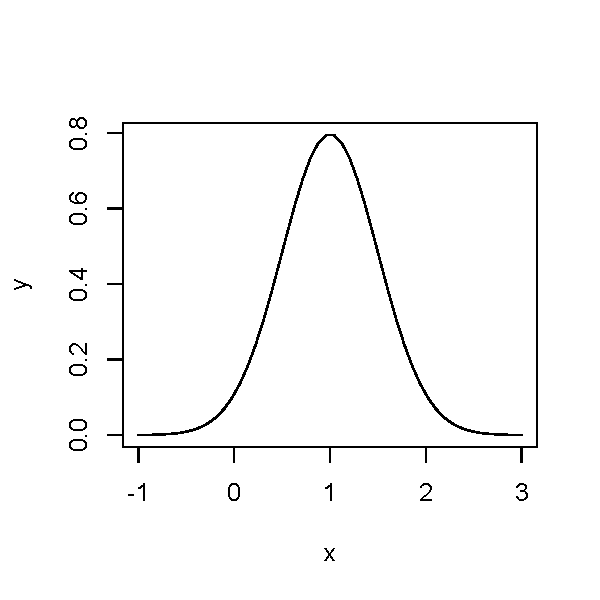
\includegraphics[width=.54\textwidth]{figure/pos-distrib-01a-1} 

}


\end{knitrout}

\subsection{Probabilities from parameters and quantiles}\label{sec:prob:quant}
\index{distributions!probabilities from quantiles}

If we have a calculated quantile we can look up the corresponding $p$-value from the Normal distribution. The mean and standard deviation would, in such a case, also be computed from the same observations under the null hypothesis. In the example below, we use invented values for all parameters \code{q}, the quantile, \code{mean}, and \code{sd}, the standard deviation. Use

\begin{knitrout}\footnotesize
\definecolor{shadecolor}{rgb}{0.969, 0.969, 0.969}\color{fgcolor}\begin{kframe}
\begin{alltt}
\hlkwd{pnorm}\hlstd{(}\hlkwc{q} \hlstd{=} \hlnum{4}\hlstd{,} \hlkwc{mean} \hlstd{=} \hlnum{0}\hlstd{,} \hlkwc{sd} \hlstd{=} \hlnum{1}\hlstd{)}
\end{alltt}
\begin{verbatim}
## [1] 0.9999683
\end{verbatim}
\begin{alltt}
\hlkwd{pnorm}\hlstd{(}\hlkwc{q} \hlstd{=} \hlnum{4}\hlstd{,} \hlkwc{mean} \hlstd{=} \hlnum{0}\hlstd{,} \hlkwc{sd} \hlstd{=} \hlnum{1}\hlstd{,} \hlkwc{lower.tail} \hlstd{=} \hlnum{FALSE}\hlstd{)}
\end{alltt}
\begin{verbatim}
## [1] 3.167124e-05
\end{verbatim}
\begin{alltt}
\hlkwd{pnorm}\hlstd{(}\hlkwc{q} \hlstd{=} \hlnum{4}\hlstd{,} \hlkwc{mean} \hlstd{=} \hlnum{0}\hlstd{,} \hlkwc{sd} \hlstd{=} \hlnum{4}\hlstd{,} \hlkwc{lower.tail} \hlstd{=} \hlnum{FALSE}\hlstd{)}
\end{alltt}
\begin{verbatim}
## [1] 0.1586553
\end{verbatim}
\begin{alltt}
\hlkwd{pnorm}\hlstd{(}\hlkwc{q} \hlstd{=} \hlkwd{c}\hlstd{(}\hlnum{2}\hlstd{,} \hlnum{4}\hlstd{),} \hlkwc{mean} \hlstd{=} \hlnum{0}\hlstd{,} \hlkwc{sd} \hlstd{=} \hlnum{1}\hlstd{,} \hlkwc{lower.tail} \hlstd{=} \hlnum{FALSE}\hlstd{)}
\end{alltt}
\begin{verbatim}
## [1] 2.275013e-02 3.167124e-05
\end{verbatim}
\begin{alltt}
\hlkwd{pnorm}\hlstd{(}\hlkwc{q} \hlstd{=} \hlnum{4}\hlstd{,} \hlkwc{mean} \hlstd{=} \hlnum{0}\hlstd{,} \hlkwc{sd} \hlstd{=} \hlkwd{c}\hlstd{(}\hlnum{1}\hlstd{,} \hlnum{4}\hlstd{),} \hlkwc{lower.tail} \hlstd{=} \hlnum{FALSE}\hlstd{)}
\end{alltt}
\begin{verbatim}
## [1] 3.167124e-05 1.586553e-01
\end{verbatim}
\end{kframe}
\end{knitrout}

\begin{explainbox}
  In tests of significance, empirical $z$-values and $t$-values are computed by subtracting from the observed mean for one group or raw quantile, the ``expected'' mean (possibly a hypothesized theoretical value, the mean of a control condition used as reference, or the mean computed over all treatments under the assumption of no effect of treatments) and then dividing by the standard deviation. Consequently, the $p$-values corresponding to these empirical $z$-values and $t$-values need to be looked up using \code{mean = 0} and \code{sd = 1} when calling \Rfunction{pnorm()} or \Rfunction{pt()} respectively. These frequently used values are the defaults.
\end{explainbox}

\subsection{Quantiles from parameters and probabilities}\label{sec:quant:prob}
\index{distributions!quantiles from probabilities}

The reverse computation from that in the previous section is to obtain the quantile corresponding to a known $p$-value. These quantiles are equivalent to the values in the tables used earlier to assess significance.

\begin{knitrout}\footnotesize
\definecolor{shadecolor}{rgb}{0.969, 0.969, 0.969}\color{fgcolor}\begin{kframe}
\begin{alltt}
\hlkwd{qnorm}\hlstd{(}\hlkwc{p} \hlstd{=} \hlnum{0.01}\hlstd{,} \hlkwc{mean} \hlstd{=} \hlnum{0}\hlstd{,} \hlkwc{sd} \hlstd{=} \hlnum{1}\hlstd{)}
\end{alltt}
\begin{verbatim}
## [1] -2.326348
\end{verbatim}
\begin{alltt}
\hlkwd{qnorm}\hlstd{(}\hlkwc{p} \hlstd{=} \hlnum{0.05}\hlstd{,} \hlkwc{mean} \hlstd{=} \hlnum{0}\hlstd{,} \hlkwc{sd} \hlstd{=} \hlnum{1}\hlstd{)}
\end{alltt}
\begin{verbatim}
## [1] -1.644854
\end{verbatim}
\begin{alltt}
\hlkwd{qnorm}\hlstd{(}\hlkwc{p} \hlstd{=} \hlnum{0.05}\hlstd{,} \hlkwc{mean} \hlstd{=} \hlnum{0}\hlstd{,} \hlkwc{sd} \hlstd{=} \hlnum{1}\hlstd{,} \hlkwc{lower.tail} \hlstd{=} \hlnum{FALSE}\hlstd{)}
\end{alltt}
\begin{verbatim}
## [1] 1.644854
\end{verbatim}
\end{kframe}
\end{knitrout}

\begin{warningbox}
Quantile functions like \Rfunction{qnorm()} and probability functions like \Rfunction{pnorm()} always do computations based on a single tail of the distribution, even though it is possible to specify which tail we are interested in. If we are interested in obtaining simultaneous quantiles for both tails, we need to do this manually. If we are aiming at quantiles for $P = 0.05$, we need to find the quantile for each tail based on $P / 2 = 0.025$.

\begin{knitrout}\footnotesize
\definecolor{shadecolor}{rgb}{0.969, 0.969, 0.969}\color{fgcolor}\begin{kframe}
\begin{alltt}
\hlkwd{qnorm}\hlstd{(}\hlkwc{p} \hlstd{=} \hlnum{0.025}\hlstd{,} \hlkwc{mean} \hlstd{=} \hlnum{0}\hlstd{,} \hlkwc{sd} \hlstd{=} \hlnum{1}\hlstd{)}
\end{alltt}
\begin{verbatim}
## [1] -1.959964
\end{verbatim}
\begin{alltt}
\hlkwd{qnorm}\hlstd{(}\hlkwc{p} \hlstd{=} \hlnum{0.025}\hlstd{,} \hlkwc{mean} \hlstd{=} \hlnum{0}\hlstd{,} \hlkwc{sd} \hlstd{=} \hlnum{1}\hlstd{,} \hlkwc{lower.tail} \hlstd{=} \hlnum{FALSE}\hlstd{)}
\end{alltt}
\begin{verbatim}
## [1] 1.959964
\end{verbatim}
\end{kframe}
\end{knitrout}

We see above that in the case of a symmetric distribution like the Normal, the quantiles in the two tails differ only in sign. This is not the case for asymmetric distributions.

When calculating a $p$-value from a quantile in a test of significance, we need to first decide whether a two-sided or single-sided test is relevant, and in the case of a single sided test, which tail is of interest. For a two-sided test we need to multiply the returned value by 2.

\begin{knitrout}\footnotesize
\definecolor{shadecolor}{rgb}{0.969, 0.969, 0.969}\color{fgcolor}\begin{kframe}
\begin{alltt}
\hlkwd{pnorm}\hlstd{(}\hlkwc{q} \hlstd{=} \hlnum{4}\hlstd{,} \hlkwc{mean} \hlstd{=} \hlnum{0}\hlstd{,} \hlkwc{sd} \hlstd{=} \hlnum{1}\hlstd{)} \hlopt{*} \hlnum{2}
\end{alltt}
\begin{verbatim}
## [1] 1.999937
\end{verbatim}
\end{kframe}
\end{knitrout}

\end{warningbox}

\subsection{``Random'' draws from a distribution}\label{sec:stat:random}
\index{random draws|see{distributions!pseudo-random draws}}\index{distributions!pseudo-random draws}

True random sequences can only be generated by physical processes. All so-called ``random'' sequences of numbers generated by computation are really deterministic although they share some properties with true random sequences (e.g.,  in relation to autocorrelation). It is possible to compute not only pseudo-random draws from a uniform distribution but also from the Normal, $t$, $F$ and other distributions. Parameter \code{n} indicates the number of values to be drawn, or its equivalent, the length of the vector returned.\qRfunction{rnorm()}\qRfunction{runif()}

\begin{knitrout}\footnotesize
\definecolor{shadecolor}{rgb}{0.969, 0.969, 0.969}\color{fgcolor}\begin{kframe}
\begin{alltt}
\hlkwd{rnorm}\hlstd{(}\hlnum{5}\hlstd{)}
\end{alltt}
\begin{verbatim}
## [1] -0.8248801  0.1201213 -0.4787266 -0.7134216  1.1264443
\end{verbatim}
\begin{alltt}
\hlkwd{rnorm}\hlstd{(}\hlkwc{n} \hlstd{=} \hlnum{10}\hlstd{,} \hlkwc{mean} \hlstd{=} \hlnum{10}\hlstd{,} \hlkwc{sd} \hlstd{=} \hlnum{2}\hlstd{)}
\end{alltt}
\begin{verbatim}
##  [1] 12.394190  9.697729  9.212345 11.624844 12.194317 10.257707 10.082981
##  [8] 10.268540 10.792963  7.772915
\end{verbatim}
\end{kframe}
\end{knitrout}

\begin{playground}
Edit the examples in sections \ref{sec:prob:quant}, \ref{sec:quant:prob} and \ref{sec:stat:random} to do computations based on different distributions, such as Student's \emph{t}, \emph{F} or uniform.
\end{playground}

\begin{explainbox}
\index{random numbers|see{pseudo-random numbers}}\index{pseudo-random numbers}
It is impossible to generate truly random sequences of numbers by means of a deterministic process such as a mathematical computation. ``Random numbers'' as generated by \Rpgrm and other computer programs are \emph{pseudo random numbers}, long deterministic series of numbers that resemble random draws. Random number generation uses a \emph{seed} value that determines where in the series we start. The usual way of automatically setting the value of the seed is to take the milliseconds or similar rapidly changing set of digits from the real time clock of the computer. However, in cases when we wish to repeat a calculation using the same series of pseudo-random values, we can use \Rfunction{set.seed()} with an arbitrary integer as an argument to reset the generator to the same point in the underlying (deterministic) sequence.
\end{explainbox}

\begin{advplayground}
Execute the statement \code{rnorm(3)}\qRfunction{rnorm()} by itself several times, paying attention to the values obtained. Repeat the exercise, but now executing \code{set.seed(98765)}\qRfunction{setseed()} immediately before each call to \code{rnorm(3)}, again paying attention to the values obtained. Next execute \code{set.seed(98765)}, followed by \code{c(rnorm(3), rnorm(3))}, and then execute \code{set.seed(98765)}, followed by \code{rnorm(6)} and compare the output. Repeat the exercise using a different argument in the call to \code{set.seed()}. analyze the results and explain how \code{setseed()} affects the generation of pseudo-random numbers in \Rlang.
\end{advplayground}

\section{``Random'' sampling}
\index{random sampling|see{pseudo-random sampling}}%
\index{pseudo-random sampling}%

In addition to drawing values from a theoretical distribution, we can draw values from an existing set or collection of values. We call this operation (pseudo-)random sampling. The draws can be done either with replacement or without replacement. In the second case, all draws are taken from the whole set of values, making it possible for a given value to be drawn more than once. In the default case of not using replacement, subsequent draws are taken from the values remaining after removing the values chosen in earlier draws.

\begin{knitrout}\footnotesize
\definecolor{shadecolor}{rgb}{0.969, 0.969, 0.969}\color{fgcolor}\begin{kframe}
\begin{alltt}
\hlkwd{sample}\hlstd{(}\hlkwc{x} \hlstd{= LETTERS)}
\end{alltt}
\begin{verbatim}
##  [1] "Z" "N" "Y" "R" "M" "E" "W" "J" "H" "G" "U" "O" "S" "T" "L" "F" "X" "P" "K"
## [20] "V" "D" "A" "B" "C" "I" "Q"
\end{verbatim}
\begin{alltt}
\hlkwd{sample}\hlstd{(}\hlkwc{x} \hlstd{= LETTERS,} \hlkwc{size} \hlstd{=} \hlnum{12}\hlstd{)}
\end{alltt}
\begin{verbatim}
##  [1] "M" "S" "L" "R" "B" "D" "Q" "W" "V" "N" "J" "P"
\end{verbatim}
\begin{alltt}
\hlkwd{sample}\hlstd{(}\hlkwc{x} \hlstd{= LETTERS,} \hlkwc{size} \hlstd{=} \hlnum{12}\hlstd{,} \hlkwc{replace} \hlstd{=} \hlnum{TRUE}\hlstd{)}
\end{alltt}
\begin{verbatim}
##  [1] "K" "E" "V" "N" "A" "Q" "L" "C" "T" "L" "H" "U"
\end{verbatim}
\end{kframe}
\end{knitrout}

In practice, pseudo-random sampling is useful when we need to select subsets of observations. One such case is  assigning treatments to experimental units in an experiment or selecting persons to interview in a survey. Another use is in bootstrapping to estimate variation in parameter estimates using empirical distributions.
\index{distributions|)}

\section{Correlation}
\index{correlation|(}
Both parametric (Pearson's) and non-parametric robust (Spearman's and Kendall's) methods for the estimation of the (linear) correlation between pairs of variables are available in base \Rlang. The different methods are selected by passing arguments to a single function. While Pearson's method is based on the actual values of the observations, non-parametric methods are based on the ordering or rank of the observations, and consequently less affected by observations with extreme values.

We first load and explore the data set \Rdata{cars} from \Rlang which we will use in the example. These data consist of stopping distances for cars moving at different speeds as described in the documentation available by entering \code{help(cars)}).

\begin{knitrout}\footnotesize
\definecolor{shadecolor}{rgb}{0.969, 0.969, 0.969}\color{fgcolor}\begin{kframe}
\begin{alltt}
\hlkwd{data}\hlstd{(cars)}
\hlkwd{plot}\hlstd{(cars)}
\end{alltt}
\end{kframe}

{\centering 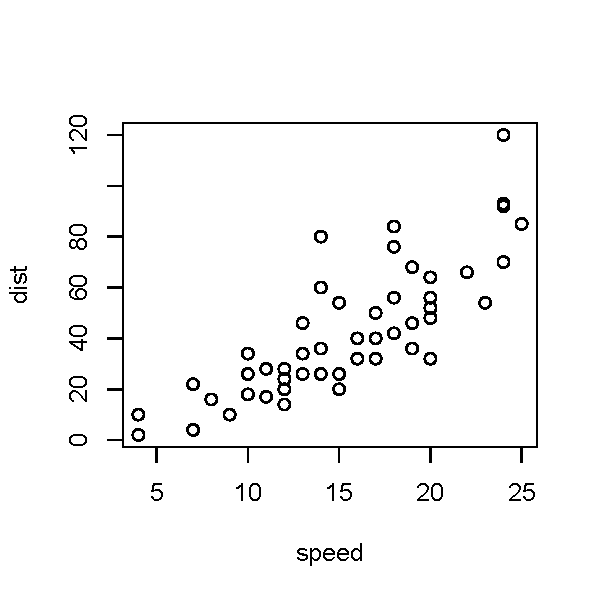
\includegraphics[width=.54\textwidth]{figure/pos-cor-00-1} 

}


\end{knitrout}
\label{chunk:plot:cars}

\subsection{Pearson's $r$}
\index{correlation!parametric}
\index{correlation!Pearson}

Function \Rfunction{cor()} can be called with two vectors of the same length as arguments. In the case of the parametric Pearson method, we do not need to provide further arguments as this method is the default one.

\begin{knitrout}\footnotesize
\definecolor{shadecolor}{rgb}{0.969, 0.969, 0.969}\color{fgcolor}\begin{kframe}
\begin{alltt}
\hlkwd{cor}\hlstd{(}\hlkwc{x} \hlstd{= cars}\hlopt{$}\hlstd{speed,} \hlkwc{y} \hlstd{= cars}\hlopt{$}\hlstd{dist)}
\end{alltt}
\begin{verbatim}
## [1] 0.8068949
\end{verbatim}
\end{kframe}
\end{knitrout}

It is also possible to pass a data frame (or a matrix) as the only argument. When the data frame (or matrix) contains only two columns, the returned value is equivalent to that of passing the two columns individually as vectors.

\begin{knitrout}\footnotesize
\definecolor{shadecolor}{rgb}{0.969, 0.969, 0.969}\color{fgcolor}\begin{kframe}
\begin{alltt}
\hlkwd{cor}\hlstd{(cars)}
\end{alltt}
\begin{verbatim}
##           speed      dist
## speed 1.0000000 0.8068949
## dist  0.8068949 1.0000000
\end{verbatim}
\end{kframe}
\end{knitrout}

When the data frame or matrix contains more than two numeric vectors, the returned value is a matrix of estimates of pairwise correlations between columns. We here use \Rfunction{rnorm()} described above to create a long vector of pseudo-random values drawn from the Normal distribution and \Rfunction{matrix()} to convert it into a matrix with three columns (see page \pageref{sec:matrix:array} for details about \Rlang matrices).

\begin{knitrout}\footnotesize
\definecolor{shadecolor}{rgb}{0.969, 0.969, 0.969}\color{fgcolor}\begin{kframe}
\begin{alltt}
\hlstd{my.mat} \hlkwb{<-} \hlkwd{matrix}\hlstd{(}\hlkwd{rnorm}\hlstd{(}\hlnum{54}\hlstd{),} \hlkwc{ncol} \hlstd{=} \hlnum{3}\hlstd{,}
                 \hlkwc{dimnames} \hlstd{=} \hlkwd{list}\hlstd{(}\hlkwc{rows} \hlstd{=} \hlnum{1}\hlopt{:}\hlnum{18}\hlstd{,} \hlkwc{cols} \hlstd{=} \hlkwd{c}\hlstd{(}\hlstr{"A"}\hlstd{,} \hlstr{"B"}\hlstd{,} \hlstr{"C"}\hlstd{)))}
\hlkwd{cor}\hlstd{(my.mat)}
\end{alltt}
\begin{verbatim}
##            A         B          C
## A 1.00000000 0.2126595 0.05623007
## B 0.21265951 1.0000000 0.31065243
## C 0.05623007 0.3106524 1.00000000
\end{verbatim}
\end{kframe}
\end{knitrout}

\begin{playground}
Modify the code in the chunk immediately above constructing a matrix with six columns and then computing the correlations.
\end{playground}

While \Rfunction{cor()} returns and estimate for $r$ the correlation coefficient, \Rfunction{cor.test()} also computes the $t$-value, $p$-value, and confidence interval for the estimate.

\begin{knitrout}\footnotesize
\definecolor{shadecolor}{rgb}{0.969, 0.969, 0.969}\color{fgcolor}\begin{kframe}
\begin{alltt}
\hlkwd{cor.test}\hlstd{(}\hlkwc{x} \hlstd{= cars}\hlopt{$}\hlstd{speed,} \hlkwc{y} \hlstd{= cars}\hlopt{$}\hlstd{dist)}
\end{alltt}
\begin{verbatim}
## 
## 	Pearson's product-moment correlation
## 
## data:  cars$speed and cars$dist
## t = 9.464, df = 48, p-value = 1.49e-12
## alternative hypothesis: true correlation is not equal to 0
## 95 percent confidence interval:
##  0.6816422 0.8862036
## sample estimates:
##       cor 
## 0.8068949
\end{verbatim}
\end{kframe}
\end{knitrout}

As described below for model fitting and $t$-test, \Rfunction{cor.test()} also accepts a \code{formula} plus \code{data} as arguments.

\begin{playground}
Functions \Rfunction{cor()} and \Rfunction{cor.test()} return \Rlang objects, that when using \Rlang interactively get automatically ``printed'' on the screen. One should be aware that \Rfunction{print()} methods do not necessarily display all the information contained in an \Rlang object. This is almost always the case for complex objects like those returned by \Rlang functions implementing statistical tests. As with any \Rlang object we can save the result of an analysis into a variable. As described in section \ref{sec:calc:lists} on page \pageref{sec:calc:lists} for lists, we can peek into the structure of an object with method \Rfunction{str()}. We can use \Rfunction{class()} and \Rfunction{attributes()} to extract further information. Run the code in the chunk below to discover what is actually returned by \Rfunction{cor()}.

\begin{knitrout}\footnotesize
\definecolor{shadecolor}{rgb}{0.969, 0.969, 0.969}\color{fgcolor}\begin{kframe}
\begin{alltt}
\hlstd{a} \hlkwb{<-} \hlkwd{cor}\hlstd{(cars)}
\hlkwd{class}\hlstd{(a)}
\hlkwd{attributes}\hlstd{(a)}
\hlkwd{str}\hlstd{(a)}
\end{alltt}
\end{kframe}
\end{knitrout}

Methods \Rfunction{class()}, \Rfunction{attributes()} and \Rfunction{str()} are very powerful tools that can be used when we are in doubt about the data contained in an object and/or how it is structured. Knowing the structure allows us to retrieve the data members directly from the object when predefined extractor methods are not available.
\end{playground}

\subsection{Kendall's $\tau$ and Spearman's $\rho$}
\index{correlation!non-parametric}
\index{correlation!Kendall}
\index{correlation!Spearman}

We use the same functions as for Pearson's $r$ but explicitly request the use of one of these methods by passing and argument.

\begin{knitrout}\footnotesize
\definecolor{shadecolor}{rgb}{0.969, 0.969, 0.969}\color{fgcolor}\begin{kframe}
\begin{alltt}
\hlkwd{cor}\hlstd{(}\hlkwc{x} \hlstd{= cars}\hlopt{$}\hlstd{speed,} \hlkwc{y} \hlstd{= cars}\hlopt{$}\hlstd{dist,} \hlkwc{method} \hlstd{=} \hlstr{"kendall"}\hlstd{)}
\end{alltt}
\begin{verbatim}
## [1] 0.6689901
\end{verbatim}
\begin{alltt}
\hlkwd{cor}\hlstd{(}\hlkwc{x} \hlstd{= cars}\hlopt{$}\hlstd{speed,} \hlkwc{y} \hlstd{= cars}\hlopt{$}\hlstd{dist,} \hlkwc{method} \hlstd{=} \hlstr{"spearman"}\hlstd{)}
\end{alltt}
\begin{verbatim}
## [1] 0.8303568
\end{verbatim}
\end{kframe}
\end{knitrout}

Function \Rfunction{cor.test()}, described above, also allows the choice of method with the same syntax as shown for \Rfunction{cor()}.

\begin{playground}
Repeat the exercise in the playground immediately above, but now using non-parametric methods. How does the information stored in the returned \code{matrix} differ depending on the method, and how can we extract information about the method used for calculation of the correlation from the returned object.
\end{playground}
\index{correlation|)}

\section[Model fitting in R]{Model fitting in \Rlang}\label{sec:stat:mf}
\index{models fitting|(}
The general approach to model fitting in \Rlang is to separate the actual fitting of a model from the inspection of the fitted model. A model fitting function minimally requires a description of the model to fit, as a model \code{formula} and a data frame or vectors with the data or observations to which to fit the model. These functions in \Rlang return a model fit object. This object contains the data, the model formula, call and the result of fitting the model. To inspect this model several methods are available. In the diagram we show a linear model fit, done with function \Rfunction{lm()} where the non-filled boxes represent what is in common with the fitting of other types of models, and the filled ones what is specific to \Rfunction{lm()}.

\begin{center}
\begin{small}
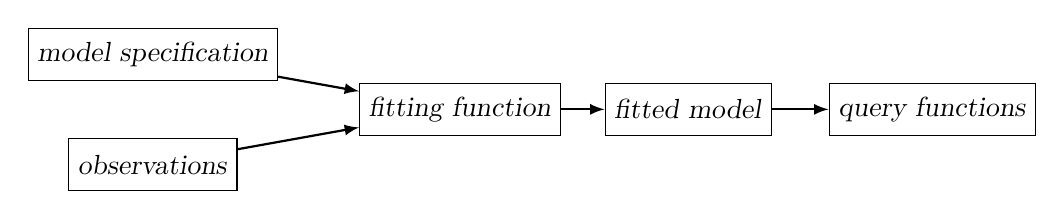
\begin{tikzpicture}[node distance=1.4cm, scale=0.5]
\node (model) [tprocess] {\textsl{model specification}};
\node (data) [tprocess, below of=model] {\textsl{observations}};
\node (fitfun) [tprocess, right of=model, yshift=-0.7cm, xshift=2.5cm] {\textsl{fitting function}};
\node (fm) [tprocess, color = black, right of=fitfun, xshift=1.5cm] {\textsl{fitted model}};
\node (summary) [tprocess, color = black, right of=fm, xshift=1.7cm] {\textsl{query functions}};
\draw [arrow] (model) -- (fitfun);
\draw [arrow] (data) -- (fitfun);
\draw [arrow] (fitfun) -- (fm);
\draw [arrow] (fm) -- (summary);
\end{tikzpicture}
\end{small}
\end{center}

Models are described using model formulas such as \verb|y ~ x| which we read as $y$ is explained by $x$. We use lhs (left-hand-side) and rhs (right-hand-side) to signify all terms to the left and right of the tilde (\verb|~|), respectively (\verb|<lhs> ~ <rhs>|). Model formulas are used in different contexts: fitting of models, plotting, and tests like $t$-test. The syntax of model formulas is consistent throughout base \Rlang and numerous independently developed packages. However, their use is not universal, and several packages extend the basic syntax to allow the description of specific types of models. As most things in \Rlang, model formulas are objects and can be stored in variables. See section \ref{sec:stat:formulas} on page \pageref{sec:stat:formulas} for a detailed discussion of models formulas.

Although there is some variation, especially for fitted model classes defined in extension packages, in most cases to the \textsl{query functions} bulked together in rightmost box in the diagram include methods \Rfunction{summary()}, \Rfunction{anova()} and \Rfunction{plot()}, with several other methods such as \Rfunction{coef()}, \Rfunction{residuals()}, \Rfunction{fitted()}, \Rfunction{predict()}, \Rfunction{AIC()}, \Rfunction{BIC()} usually also available. Additional methods may be available. However, as model fit object are derived from class \code{list}, these and other components can be extract or computed programmatically. Consequently, the examples in this chapter can be adapted to the fitting of types of models not described here.

\begin{explainbox}
  Fitted model objects in \Rlang are self contained and include a copy of the data to which the model was fit, as well as residuals and possibly even intermediate results of computations. Although this can make the size of these objects large, it allows querying and even updating them in the absence of the data in the current \Rlang workspace.
\end{explainbox}

\index{models fitting|)}

\section{Fitting linear models}\label{sec:stat:LM}
\index{models!linear|see{linear models}}
\index{linear models|(}
\index{LM|see{linear models}}

The \Rlang function \Rfunction{lm()} is used to fit linear models. If the explanatory variable is continuous, the fit is a regression. If the explanatory variable is a factor, the fit is an analysis of variance (ANOVA) in broad terms. However, there is another meaning of ANOVA, referring only to the tests of significance rather to an approach to model fitting. Consequently, rather confusingly, results for tests of significance for fitted parameter estimates can both in the case of regression and ANOVA, be presented in an ANOVA table. In this second, stricter meaning, ANOVA means a test of significance based on the ratios between pairs of variances.

\begin{warningbox}
If you do not clearly remember the difference between numeric vectors and factors, or how they can be created, please, revisit chapter \ref{chap:R:as:calc} on page \pageref{chap:R:as:calc}.
\end{warningbox}

The generic diagram from the previous section redrawn to show a linear model fit, done with function \Rfunction{lm()} where the non-filled boxes represent what is in common with the fitting of other types of models, and the filled ones what is specific to \Rfunction{lm()}.

\begin{center}
\begin{small}
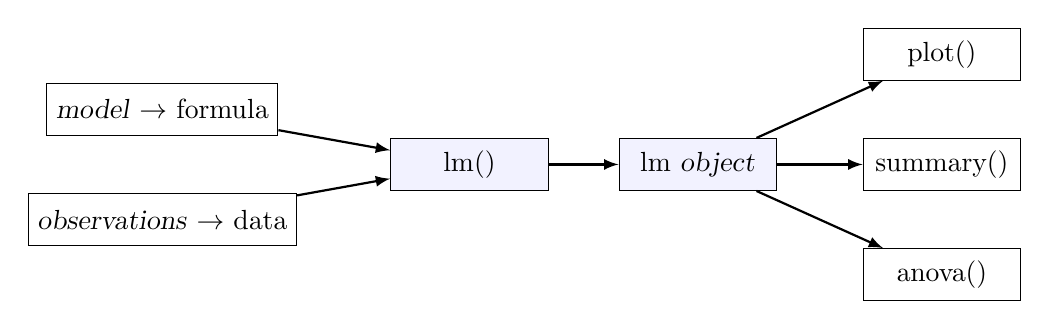
\begin{tikzpicture}[node distance=1.4cm, scale=0.5]
\node (model) [tprocess] {\textsl{model} $\to$ \code{formula}};
\node (data) [tprocess, below of=model] {\textsl{observations} $\to$ \code{data}};
\node (fitfun) [tprocess, right of=model, yshift=-0.7cm, xshift=2.5cm, fill=blue!5] {\code{lm()}};
\node (fm) [tprocess, color = black, right of=fitfun, xshift=1.5cm, fill=blue!5] {\code{lm} \textsl{object}};
\node (summary) [tprocess, color = black, right of=fm, xshift=1.7cm] {\code{summary()}};
\node (anova) [tprocess, color = black, below of=summary] {\code{anova()}};
\node (plot) [tprocess, color = black, above of=summary] {\code{plot()}};
\draw [arrow] (model) -- (fitfun);
\draw [arrow] (data) -- (fitfun);
\draw [arrow] (fitfun) -- (fm);
\draw [arrow] (fm) -- (plot);
\draw [arrow] (fm) -- (anova);
\draw [arrow] (fm) -- (summary);
\end{tikzpicture}
\end{small}
\end{center}

\subsection{Regression}
%\index{linear regression}
\index{linear regression|see{linear models!linear regression}}\index{linear models!linear regression}
In \index{linear models!ANOVA table} the example immediately below, \code{speed} is a continuous numeric variable. In the ANOVA table calculated for the model fit, in this case a linear regression, we can see that the term for \code{speed} has only one degree of freedom (df).

In the next example we continue using the stopping distance for \Rdata{cars} data set included in \Rpgrm. Please see the plot on page \pageref{chunk:plot:cars}.
\label{xmpl:fun:lm:fm1}

\begin{knitrout}\footnotesize
\definecolor{shadecolor}{rgb}{0.969, 0.969, 0.969}\color{fgcolor}\begin{kframe}
\begin{alltt}
\hlkwd{data}\hlstd{(cars)}
\hlkwd{is.factor}\hlstd{(cars}\hlopt{$}\hlstd{speed)}
\end{alltt}
\begin{verbatim}
## [1] FALSE
\end{verbatim}
\begin{alltt}
\hlkwd{is.numeric}\hlstd{(cars}\hlopt{$}\hlstd{speed)}
\end{alltt}
\begin{verbatim}
## [1] TRUE
\end{verbatim}
\end{kframe}
\end{knitrout}

We then fit the simple linear model $y = \alpha \cdot 1 + \beta \cdot x$ where $y$ corresponds to stopping distance (\code{dist}) and $x$ to initial speed (\code{speed}). Such a model is formulated in \Rlang as \verb|dist ~ 1 + speed|. We save the fitted model as \code{fm1} (a mnemonic for fitted-model one).\label{chunk:lm:models1}

\begin{knitrout}\footnotesize
\definecolor{shadecolor}{rgb}{0.969, 0.969, 0.969}\color{fgcolor}\begin{kframe}
\begin{alltt}
\hlstd{fm1} \hlkwb{<-} \hlkwd{lm}\hlstd{(dist} \hlopt{~} \hlnum{1} \hlopt{+} \hlstd{speed,} \hlkwc{data}\hlstd{=cars)}
\hlkwd{class}\hlstd{(fm1)}
\end{alltt}
\begin{verbatim}
## [1] "lm"
\end{verbatim}
\end{kframe}
\end{knitrout}

The next step is diagnosis of the fit. Are assumptions of the linear model procedure used reasonably close to being fulfilled? In \Rlang it is most common to use plots to this end. We show here only one of the four plots normally produced. This quantile vs.\ quantile plot allows us to assess how much the residuals deviate from being normally distributed.

\begin{knitrout}\footnotesize
\definecolor{shadecolor}{rgb}{0.969, 0.969, 0.969}\color{fgcolor}\begin{kframe}
\begin{alltt}
\hlkwd{plot}\hlstd{(fm1,} \hlkwc{which} \hlstd{=} \hlnum{2}\hlstd{)}
\end{alltt}
\end{kframe}

{\centering 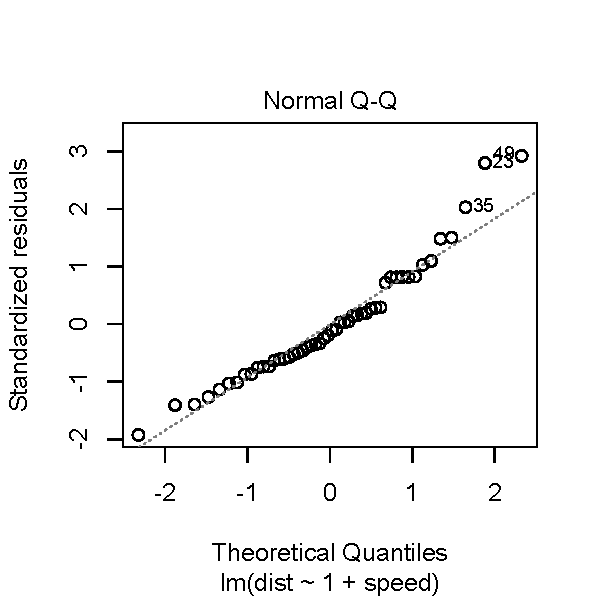
\includegraphics[width=.54\textwidth]{figure/pos-models-1a-1} 

}


\end{knitrout}

In the case of a regression, calling \Rfunction{summary()} with the fitted model object as argument is most useful as it provides a table of coefficient estimates and their errors. Remember that as is the case for most \Rlang functions, the value returned by \Rfunction{summary()} is printed when we call this method at the \Rlang prompt.

\begin{knitrout}\footnotesize
\definecolor{shadecolor}{rgb}{0.969, 0.969, 0.969}\color{fgcolor}\begin{kframe}
\begin{alltt}
\hlkwd{summary}\hlstd{(fm1)}
\end{alltt}
\begin{verbatim}
## 
## Call:
## lm(formula = dist ~ 1 + speed, data = cars)
## 
## Residuals:
##     Min      1Q  Median      3Q     Max 
## -29.069  -9.525  -2.272   9.215  43.201 
## 
## Coefficients:
##             Estimate Std. Error t value Pr(>|t|)    
## (Intercept) -17.5791     6.7584  -2.601   0.0123 *  
## speed         3.9324     0.4155   9.464 1.49e-12 ***
## ---
## Signif. codes:  0 '***' 0.001 '**' 0.01 '*' 0.05 '.' 0.1 ' ' 1
## 
## Residual standard error: 15.38 on 48 degrees of freedom
## Multiple R-squared:  0.6511,	Adjusted R-squared:  0.6438 
## F-statistic: 89.57 on 1 and 48 DF,  p-value: 1.49e-12
\end{verbatim}
\end{kframe}
\end{knitrout}

Let's\index{linear models!summary table} look at the printout of the summary, section by section. Under ``Call:'' we find, \verb|dist ~ 1 + speed| or the specification of the model fitted, plus the data used. Under ``Residuals:'' we find the extremes, quartiles and median of the residuals, or deviations between observations and the fitted line. Under ``Coefficients:'' we find the estimates of the model parameters and their variation plus corresponding $t$-tests. At the end of the summary there is information on degrees of freedom and overall coefficient of determination ($R^2$).

If we return to the model formulation, we can now replace $\alpha$ and $\beta$ by the estimates obtaining $y = -17.6 + 3.93 x$. Given the nature of the problem, we \emph{know based on first principles} that stopping distance must be zero when speed is zero. This suggests that we should not estimate the value of $\alpha$ but instead set $\alpha = 0$, or in other words, fit the model $y = \beta \cdot x$.

However, in \Rlang models, the intercept is always implicitly included, so the model fitted above can be formulated as \verb|dist ~ speed|---i.e., a missing \code{+ 1} does not change the model. To exclude the intercept from the previous model, we need to specify it as \verb|dist ~ speed - 1| (or its equivalent \verb|dist ~ speed + 0|), resulting in the fitting of a straight line passing through the origin ($x = 0$, $y = 0$).

\begin{knitrout}\footnotesize
\definecolor{shadecolor}{rgb}{0.969, 0.969, 0.969}\color{fgcolor}\begin{kframe}
\begin{alltt}
\hlstd{fm2} \hlkwb{<-} \hlkwd{lm}\hlstd{(dist} \hlopt{~} \hlstd{speed} \hlopt{-} \hlnum{1}\hlstd{,} \hlkwc{data} \hlstd{= cars)}
\hlkwd{summary}\hlstd{(fm2)}
\end{alltt}
\begin{verbatim}
## 
## Call:
## lm(formula = dist ~ speed - 1, data = cars)
## 
## Residuals:
##     Min      1Q  Median      3Q     Max 
## -26.183 -12.637  -5.455   4.590  50.181 
## 
## Coefficients:
##       Estimate Std. Error t value Pr(>|t|)    
## speed   2.9091     0.1414   20.58   <2e-16 ***
## ---
## Signif. codes:  0 '***' 0.001 '**' 0.01 '*' 0.05 '.' 0.1 ' ' 1
## 
## Residual standard error: 16.26 on 49 degrees of freedom
## Multiple R-squared:  0.8963,	Adjusted R-squared:  0.8942 
## F-statistic: 423.5 on 1 and 49 DF,  p-value: < 2.2e-16
\end{verbatim}
\end{kframe}
\end{knitrout}

Now there is no estimate for the intercept in the summary, only an estimate for the slope.

\begin{knitrout}\footnotesize
\definecolor{shadecolor}{rgb}{0.969, 0.969, 0.969}\color{fgcolor}\begin{kframe}
\begin{alltt}
\hlkwd{plot}\hlstd{(fm2,} \hlkwc{which} \hlstd{=} \hlnum{1}\hlstd{)}
\end{alltt}
\end{kframe}

{\centering 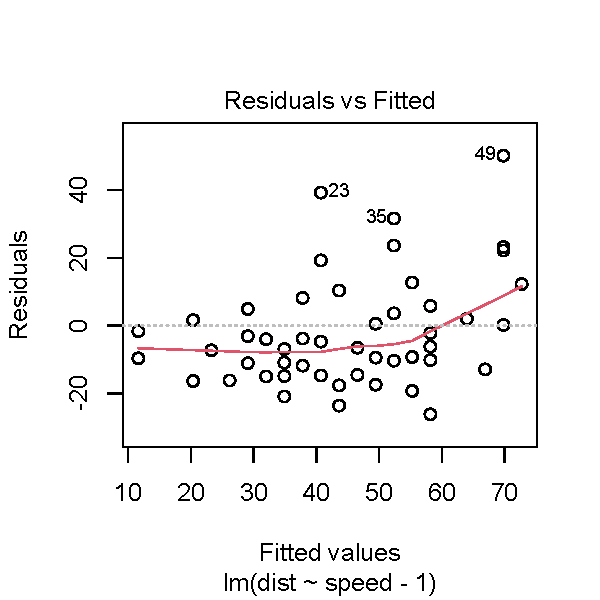
\includegraphics[width=.54\textwidth]{figure/pos-models-2a-1} 

}


\end{knitrout}

The equation of the second fitted model is $y = 2.91 x$, and from the residuals, it can be seen that it is inadequate, as the straight line does not follow the curvature of the relationship between \code{dist} and \code{speed}.

\begin{playground}
You will now fit a second-degree polynomial\index{linear models!polynomial regression}\index{polynomial regression}, a different linear model: $y = \alpha \cdot 1 + \beta_1 \cdot x + \beta_2 \cdot x^2$. The function used is the same as for linear regression, \Rfunction{lm()}. We only need to alter the formulation of the model. The identity function \Rfunction{I()} is used to protect its argument from being interpreted as part of the model formula. Instead, its argument is evaluated beforehand and the result is used as the, in this case second, explanatory variable.

\begin{knitrout}\footnotesize
\definecolor{shadecolor}{rgb}{0.969, 0.969, 0.969}\color{fgcolor}\begin{kframe}
\begin{alltt}
\hlstd{fm3} \hlkwb{<-} \hlkwd{lm}\hlstd{(dist} \hlopt{~} \hlstd{speed} \hlopt{+} \hlkwd{I}\hlstd{(speed}\hlopt{^}\hlnum{2}\hlstd{),} \hlkwc{data} \hlstd{= cars)}
\hlkwd{plot}\hlstd{(fm3,} \hlkwc{which} \hlstd{=} \hlnum{3}\hlstd{)}
\hlkwd{summary}\hlstd{(fm3)}
\hlkwd{anova}\hlstd{(fm3)}
\end{alltt}
\end{kframe}
\end{knitrout}

The ``same'' fit using an orthogonal polynomial can be specified using function \Rfunction{poly()}. Polynomials of different degrees can be obtained by supplying as the second argument to \Rfunction{poly()} the corresponding positive integer value. In this case, the different terms of the polynomial are bulked together in the summary.

\begin{knitrout}\footnotesize
\definecolor{shadecolor}{rgb}{0.969, 0.969, 0.969}\color{fgcolor}\begin{kframe}
\begin{alltt}
\hlstd{fm3a} \hlkwb{<-} \hlkwd{lm}\hlstd{(dist} \hlopt{~} \hlkwd{poly}\hlstd{(speed,} \hlnum{2}\hlstd{),} \hlkwc{data} \hlstd{= cars)}
\hlkwd{summary}\hlstd{(fm3a)}
\hlkwd{anova}\hlstd{(fm3a)}
\end{alltt}
\end{kframe}
\end{knitrout}

We can also compare two model fits using \Rfunction{anova()}, to test whether one of the models describes the data better than the other. It is important in this case to take into consideration the nature of the difference between the model formulas, most importantly if they can be interpreted as nested---i.e., interpreted as a base model vs. the same model with additional terms.

\begin{knitrout}\footnotesize
\definecolor{shadecolor}{rgb}{0.969, 0.969, 0.969}\color{fgcolor}\begin{kframe}
\begin{alltt}
\hlkwd{anova}\hlstd{(fm2, fm1)}
\end{alltt}
\end{kframe}
\end{knitrout}

Three or more models can also be compared in a single call to \Rfunction{anova()}. However, be careful, as the order of the arguments matters.

\begin{knitrout}\footnotesize
\definecolor{shadecolor}{rgb}{0.969, 0.969, 0.969}\color{fgcolor}\begin{kframe}
\begin{alltt}
\hlkwd{anova}\hlstd{(fm2, fm3, fm3a)}
\hlkwd{anova}\hlstd{(fm2, fm3a, fm3)}
\end{alltt}
\end{kframe}
\end{knitrout}

We can use different criteria to choose the ``best'' model: significance based on $p$-values or information criteria (AIC, BIC). AIC (Akaike's ``An Information Criterion'') and BIC (``Bayesian Information Criterion'' = SBC, ``Schwarz's Bayesian criterion'') that penalize the resulting ``goodness'' based on the number of parameters in the fitted model. In the case of AIC and BIC, a smaller value is better, and values returned can be either positive or negative, in which case more negative is better. Estimates for both BIC and AIC are returned by \Rfunction{anova()}, and on their own by \Rfunction{BIC()} and \Rfunction{AIC()}

\begin{knitrout}\footnotesize
\definecolor{shadecolor}{rgb}{0.969, 0.969, 0.969}\color{fgcolor}\begin{kframe}
\begin{alltt}
\hlkwd{BIC}\hlstd{(fm2, fm1, fm3, fm3a)}
\hlkwd{AIC}\hlstd{(fm2, fm1, fm3, fm3a)}
\end{alltt}
\end{kframe}
\end{knitrout}

Once you have run the code in the chunks above, you will be able see that these three criteria do not necessarily agree on which is the ``best'' model. Find in the output $p$-value, BIC and AIC estimates, for the different models and conclude which model is favored by each of the three criteria. In addition you will notice that the two different formulations of the quadratic polynomial are equivalent.

\end{playground}

Additional methods give easy access to different components of fitted models: \Rfunction{vcov()} returns the variance-covariance matrix, \Rfunction{coef()} and its alias \Rfunction{coefficients()} return the estimates for the fitted model coefficients, \Rfunction{fitted()} and its alias \Rfunction{fitted.values()} extract the fitted values, and \Rfunction{resid()} and its alias \Rfunction{residuals()} the corresponding residuals (or deviations). Less frequently used accessors are \Rfunction{effects()}, \Rfunction{terms()}, \Rfunction{model.frame()} and \Rfunction{model.matrix()}.

\begin{playground}
Familiarize yourself with these extraction and summary methods by reading their documentation and use them to explore \code{fm1} fitted above or model fits to other data of your interest.
\end{playground}

\begin{explainbox}
The objects returned by model fitting functions are rather complex and contain the full information, including the data to which the model was fit to. The different functions described above, either extract parts of the object or do additional calculations and formatting based on them. There are different specializations of these methods which are called depending on the class of the model-fit object. (See section \ref{sec:methods} on page \pageref{sec:methods}.)

\begin{knitrout}\footnotesize
\definecolor{shadecolor}{rgb}{0.969, 0.969, 0.969}\color{fgcolor}\begin{kframe}
\begin{alltt}
\hlkwd{class}\hlstd{(fm1)}
\end{alltt}
\begin{verbatim}
## [1] "lm"
\end{verbatim}
\begin{alltt}
\hlkwd{names}\hlstd{(fm1)}
\end{alltt}
\begin{verbatim}
##  [1] "coefficients"  "residuals"     "effects"       "rank"         
##  [5] "fitted.values" "assign"        "qr"            "df.residual"  
##  [9] "xlevels"       "call"          "terms"         "model"
\end{verbatim}
\end{kframe}
\end{knitrout}

We rarely need to manually explore the structure of these model-fit objects when using \Rlang interactively. In contrast, when including model fitting in scripts or package code, the need to efficiently extract specific members from them happens more frequently. As with any other \Rlang object we can use \Rfunction{str()} to explore them. As this prints as a long text, we call \Rfunction{str()} as an example, only to two components of \code{fm1} and leave to the reader the task of exploring the remaining ones.

\begin{knitrout}\footnotesize
\definecolor{shadecolor}{rgb}{0.969, 0.969, 0.969}\color{fgcolor}\begin{kframe}
\begin{alltt}
\hlkwd{str}\hlstd{(fm1}\hlopt{$}\hlstd{call)}
\end{alltt}
\begin{verbatim}
##  language lm(formula = dist ~ 1 + speed, data = cars)
\end{verbatim}
\end{kframe}
\end{knitrout}

\begin{knitrout}\footnotesize
\definecolor{shadecolor}{rgb}{0.969, 0.969, 0.969}\color{fgcolor}\begin{kframe}
\begin{alltt}
\hlkwd{str}\hlstd{(fm1}\hlopt{$}\hlstd{coefficients)}
\end{alltt}
\begin{verbatim}
##  Named num [1:2] -17.58 3.93
##  - attr(*, "names")= chr [1:2] "(Intercept)" "speed"
\end{verbatim}
\end{kframe}
\end{knitrout}

We frequently only look at the output of \Rfunction{anova()} as implicitly displayed by \code{print()}. However, both \Rfunction{anova()} and \Rfunction{summary()} return complex objects containing members with data not displayed by the matching \code{print()} methods. Understanding this is frequently useful, when we want to either display the results in a different format, or extract parts of them for use in additional tests or computations. Once again we use \Rfunction{str()} to look at the structure.

\begin{knitrout}\footnotesize
\definecolor{shadecolor}{rgb}{0.969, 0.969, 0.969}\color{fgcolor}\begin{kframe}
\begin{alltt}
\hlkwd{str}\hlstd{(}\hlkwd{anova}\hlstd{(fm1))}
\end{alltt}
\begin{verbatim}
## Classes 'anova' and 'data.frame':	2 obs. of  5 variables:
##  $ Df     : int  1 48
##  $ Sum Sq : num  21185 11354
##  $ Mean Sq: num  21185 237
##  $ F value: num  89.6 NA
##  $ Pr(>F) : num  1.49e-12 NA
##  - attr(*, "heading")= chr [1:2] "Analysis of Variance Table\n" "Response: dist"
\end{verbatim}
\end{kframe}
\end{knitrout}

The \code{coefficients} estimates are the same, but in the summary are accompanied by estimates for the corresponding standard errors, \emph{t}-value and \emph{P}-value estimates.

\begin{knitrout}\footnotesize
\definecolor{shadecolor}{rgb}{0.969, 0.969, 0.969}\color{fgcolor}\begin{kframe}
\begin{alltt}
\hlkwd{str}\hlstd{(}\hlkwd{summary}\hlstd{(fm1))}
\end{alltt}
\begin{verbatim}
## List of 11
##  $ call         : language lm(formula = dist ~ 1 + speed, data = cars)
##  $ terms        :Classes 'terms', 'formula'  language dist ~ 1 + speed
##   .. ..- attr(*, "variables")= language list(dist, speed)
##   .. ..- attr(*, "factors")= int [1:2, 1] 0 1
##   .. .. ..- attr(*, "dimnames")=List of 2
##   .. .. .. ..$ : chr [1:2] "dist" "speed"
##   .. .. .. ..$ : chr "speed"
##   .. ..- attr(*, "term.labels")= chr "speed"
##   .. ..- attr(*, "order")= int 1
##   .. ..- attr(*, "intercept")= int 1
##   .. ..- attr(*, "response")= int 1
##   .. ..- attr(*, ".Environment")=<environment: R_GlobalEnv> 
##   .. ..- attr(*, "predvars")= language list(dist, speed)
##   .. ..- attr(*, "dataClasses")= Named chr [1:2] "numeric" "numeric"
##   .. .. ..- attr(*, "names")= chr [1:2] "dist" "speed"
##  $ residuals    : Named num [1:50] 3.85 11.85 -5.95 12.05 2.12 ...
##   ..- attr(*, "names")= chr [1:50] "1" "2" "3" "4" ...
##  $ coefficients : num [1:2, 1:4] -17.579 3.932 6.758 0.416 -2.601 ...
##   ..- attr(*, "dimnames")=List of 2
##   .. ..$ : chr [1:2] "(Intercept)" "speed"
##   .. ..$ : chr [1:4] "Estimate" "Std. Error" "t value" "Pr(>|t|)"
##  $ aliased      : Named logi [1:2] FALSE FALSE
##   ..- attr(*, "names")= chr [1:2] "(Intercept)" "speed"
##  $ sigma        : num 15.4
##  $ df           : int [1:3] 2 48 2
##  $ r.squared    : num 0.651
##  $ adj.r.squared: num 0.644
##  $ fstatistic   : Named num [1:3] 89.6 1 48
##   ..- attr(*, "names")= chr [1:3] "value" "numdf" "dendf"
##  $ cov.unscaled : num [1:2, 1:2] 0.19311 -0.01124 -0.01124 0.00073
##   ..- attr(*, "dimnames")=List of 2
##   .. ..$ : chr [1:2] "(Intercept)" "speed"
##   .. ..$ : chr [1:2] "(Intercept)" "speed"
##  - attr(*, "class")= chr "summary.lm"
\end{verbatim}
\end{kframe}
\end{knitrout}

\begin{knitrout}\footnotesize
\definecolor{shadecolor}{rgb}{0.969, 0.969, 0.969}\color{fgcolor}\begin{kframe}
\begin{alltt}
\hlkwd{print}\hlstd{(}\hlkwd{summary}\hlstd{(fm1)}\hlopt{$}\hlstd{coefficients)}
\end{alltt}
\begin{verbatim}
##               Estimate Std. Error   t value     Pr(>|t|)
## (Intercept) -17.579095  6.7584402 -2.601058 1.231882e-02
## speed         3.932409  0.4155128  9.463990 1.489836e-12
\end{verbatim}
\end{kframe}
\end{knitrout}

Once we know the structure of the object and the names of members, we can simply extract them using the usual \Rlang rules for member extraction. This is useful when we need to do further calculations or when we want to present this values in a different format than that provided by the \code{print()} method, for example to add a textual annotation to a plot.

\begin{knitrout}\footnotesize
\definecolor{shadecolor}{rgb}{0.969, 0.969, 0.969}\color{fgcolor}\begin{kframe}
\begin{alltt}
\hlkwd{summary}\hlstd{(fm1)}\hlopt{$}\hlstd{adj.r.squared}
\end{alltt}
\begin{verbatim}
## [1] 0.6438102
\end{verbatim}
\end{kframe}
\end{knitrout}

As an example of a further computation, we test if the slope from a linear regression fit deviates significantly from a constant value different from the usual zero.

The examples above are for a null hypothesis of slope = 0 and next we show how to do the equivalent test with a null hypothesis of slope = 1. The procedure is applicable to any constant value as a null hypothesis for any of the fitted parameter estimates for hypotheses set \emph{a priori}. The examples use a two-sided test. In some cases, a single-sided test should be used (e.g., if its known a priori that deviation is because of physical reasons possible only in one direction away from the null hypothesis, or because only one direction of response is of interest).

To estimate the \emph{t}-value we need an estimate for the parameter and an estimate of the standard error for this estimate and its degrees of freedom.

\begin{knitrout}\footnotesize
\definecolor{shadecolor}{rgb}{0.969, 0.969, 0.969}\color{fgcolor}\begin{kframe}
\begin{alltt}
\hlstd{est.slope.value} \hlkwb{<-} \hlkwd{summary}\hlstd{(fm1)}\hlopt{$}\hlstd{coefficients[}\hlstr{"speed"}\hlstd{,} \hlstr{"Estimate"}\hlstd{]}
\hlstd{est.slope.se} \hlkwb{<-} \hlkwd{summary}\hlstd{(fm1)}\hlopt{$}\hlstd{coefficients[}\hlstr{"speed"}\hlstd{,} \hlstr{"Std. Error"}\hlstd{]}
\hlstd{degrees.of.freedom} \hlkwb{<-} \hlkwd{summary}\hlstd{(fm1)}\hlopt{$}\hlstd{df[}\hlnum{2}\hlstd{]}
\end{alltt}
\end{kframe}
\end{knitrout}

The \emph{t}-test is based on the difference between the value of the null hypothesis and the estimate.

\begin{knitrout}\footnotesize
\definecolor{shadecolor}{rgb}{0.969, 0.969, 0.969}\color{fgcolor}\begin{kframe}
\begin{alltt}
\hlstd{hyp.null} \hlkwb{<-} \hlnum{1}
\hlstd{t.value} \hlkwb{<-} \hlstd{(est.slope.value} \hlopt{-} \hlstd{hyp.null)} \hlopt{/} \hlstd{est.slope.se}
\hlstd{p.value} \hlkwb{<-} \hlkwd{dt}\hlstd{(t.value,} \hlkwc{df} \hlstd{= degrees.of.freedom)}
\hlkwd{cat}\hlstd{(}\hlstr{"t.value ="}\hlstd{,} \hlkwd{signif}\hlstd{(t.value,} \hlnum{3}\hlstd{),} \hlstr{"; P-value ="}\hlstd{,} \hlkwd{signif}\hlstd{(p.value,} \hlnum{3}\hlstd{))}
\end{alltt}
\begin{verbatim}
## t.value = 7.06 ; P-value = 1.06e-08
\end{verbatim}
\end{kframe}
\end{knitrout}

\end{explainbox}

\begin{advplayground}
Check that the procedure above agrees with the output of \code{summary()} when we set \code{hyp.null <- 0} instead of \code{hyp.null <- 1}.

Modify the example so as to test whether the intercept is significantly larger than 5 feet, doing a one-sided test.
\end{advplayground}

Method \Rfunction{predict()} uses the fitted model together with new data for the independent variables to compute predictions. As \Rfunction{predict()} accepts new data as input, it allows interpolation and extrapolation to values of the independent variables not present in the original data. In the case of fits of linear- and some other models, method \Rfunction{predict()} returns, in addition to the prediction, estimates of the confidence and/or prediction intervals. The new data must be stored in a data frame with columns using the same names for the explanatory variables as in the data used for the fit, a response variable is not needed and additional columns are ignored. (The explanatory variables in the new data can be either continuous or factors, but they must match in this respect those in the original data.)

\begin{advplayground}
Predict using both \code{fm1} and \code{fm2} the distance required to stop cars moving at 0, 5, 10, 20, 30, and 40~mph. Study the help page for the predict method for linear models (using \code{help(predict.lm)}). Explore the difference between \code{"prediction"} and \code{"confidence"} bands: why are they so different?
\end{advplayground}

\subsection{Analysis of variance, ANOVA}\label{sec:anova}
%\index{analysis of variance}
\index{analysis of variance|see{linear models!analysis of variance}}\index{linear models!analysis of variance}
\index{ANOVA|see{analysis of variance}}
We use here the \Rdata{InsectSprays} data set, giving insect counts in plots sprayed with different insecticides. In these data, \code{spray} is a factor with six levels.%
\label{xmpl:fun:lm:fm4}

The call is exactly the same as the one for linear regression, only the names of the variables and data frame are different. What determines that this is an ANOVA is that \code{spray}, the explanatory variable, is a \code{factor}.

\begin{knitrout}\footnotesize
\definecolor{shadecolor}{rgb}{0.969, 0.969, 0.969}\color{fgcolor}\begin{kframe}
\begin{alltt}
\hlkwd{data}\hlstd{(InsectSprays)}
\hlkwd{is.numeric}\hlstd{(InsectSprays}\hlopt{$}\hlstd{spray)}
\end{alltt}
\begin{verbatim}
## [1] FALSE
\end{verbatim}
\begin{alltt}
\hlkwd{is.factor}\hlstd{(InsectSprays}\hlopt{$}\hlstd{spray)}
\end{alltt}
\begin{verbatim}
## [1] TRUE
\end{verbatim}
\begin{alltt}
\hlkwd{levels}\hlstd{(InsectSprays}\hlopt{$}\hlstd{spray)}
\end{alltt}
\begin{verbatim}
## [1] "A" "B" "C" "D" "E" "F"
\end{verbatim}
\end{kframe}
\end{knitrout}

We fit the model in exactly the same way as for linear regression; the difference is that we use a factor as the explanatory variable. By using a factor instead of a numeric vector, a different model matrix is built from an equivalent formula.

\begin{knitrout}\footnotesize
\definecolor{shadecolor}{rgb}{0.969, 0.969, 0.969}\color{fgcolor}\begin{kframe}
\begin{alltt}
\hlstd{fm4} \hlkwb{<-} \hlkwd{lm}\hlstd{(count} \hlopt{~} \hlstd{spray,} \hlkwc{data} \hlstd{= InsectSprays)}
\end{alltt}
\end{kframe}
\end{knitrout}

Diagnostic plots are obtained in the same way as for linear regression.

\begin{knitrout}\footnotesize
\definecolor{shadecolor}{rgb}{0.969, 0.969, 0.969}\color{fgcolor}\begin{kframe}
\begin{alltt}
\hlkwd{plot}\hlstd{(fm4,} \hlkwc{which} \hlstd{=} \hlnum{3}\hlstd{)}
\end{alltt}
\end{kframe}

{\centering 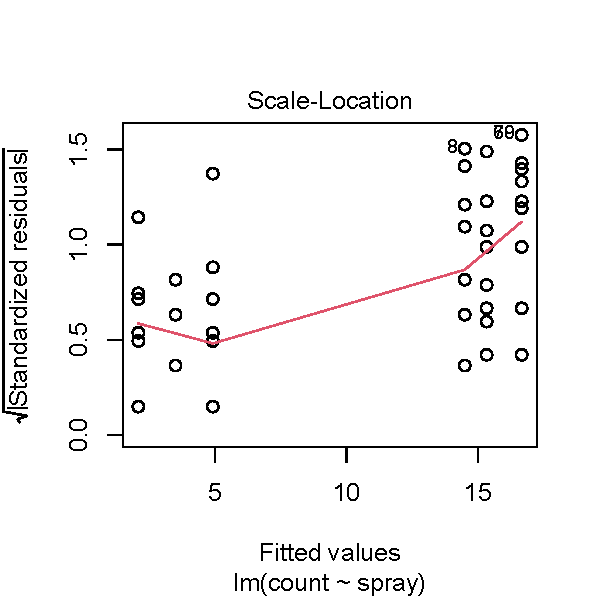
\includegraphics[width=.54\textwidth]{figure/pos-model-6a-1} 

}


\end{knitrout}

In ANOVA we are mainly interested in testing hypotheses, and \Rfunction{anova()} provides the most interesting output. Function \Rfunction{summary()} can be used to extract parameter estimates. The default contrasts and corresponding $p$-values returned by \Rfunction{summary()} test hypotheses that have little or no direct interest in an analysis of variance. Function \Rfunction{aov()} is a wrapper on \Rfunction{lm()} that returns an object that by default when printed displays the output of \Rfunction{anova()}.

\begin{knitrout}\footnotesize
\definecolor{shadecolor}{rgb}{0.969, 0.969, 0.969}\color{fgcolor}\begin{kframe}
\begin{alltt}
\hlkwd{anova}\hlstd{(fm4)}
\end{alltt}
\begin{verbatim}
## Analysis of Variance Table
## 
## Response: count
##           Df Sum Sq Mean Sq F value    Pr(>F)    
## spray      5 2668.8  533.77  34.702 < 2.2e-16 ***
## Residuals 66 1015.2   15.38                      
## ---
## Signif. codes:  0 '***' 0.001 '**' 0.01 '*' 0.05 '.' 0.1 ' ' 1
\end{verbatim}
\end{kframe}
\end{knitrout}

\begin{warningbox}
The defaults used for model fits and ANOVA calculations vary among programs. There exist different so-called ``types'' of sums of squares, usually called I, II, and III. In orthogonal designs the choice has no consequences, but differences can be important for unbalanced designs, even leading to different conclusions. \Rlang's default, type~I, is usually considered to suffer milder problems than type~III, the default used by \pgrmname{SPSS} and \pgrmname{SAS}.
\end{warningbox}

\begin{warningbox}
The contrasts used affect the estimates returned by \Rfunction{coef()} and \Rfunction{summary()} applied to an ANOVA model fit. The default used in \Rlang is different to that used in some other programs (even different than in \Slang). The default, \code{contr.treatment} uses the first level of the factor (assumed to be a control) as reference for estimation of coefficients and testing of their significance. Instead, \code{contr.sum} uses as reference the mean of all levels, i.e., using as condition that the sum of the coefficient estimates is equal to zero. Obviously this changes what the coefficients describe, and consequently also the estimated $p$-values, and most importantly how the result of the tests should be interpreted.
\end{warningbox}

The most straightforward way of setting a different default for a whole series of model fits is by setting \Rlang option \code{contrasts}, which we here only print.

\begin{knitrout}\footnotesize
\definecolor{shadecolor}{rgb}{0.969, 0.969, 0.969}\color{fgcolor}\begin{kframe}
\begin{alltt}
\hlkwd{options}\hlstd{(}\hlstr{"contrasts"}\hlstd{)}
\end{alltt}
\begin{verbatim}
## $contrasts
##         unordered           ordered 
## "contr.treatment"      "contr.poly"
\end{verbatim}
\end{kframe}
\end{knitrout}

The option is set to a named vector, with the value named \code{unordered} used when the explanatory variable is an unordered factor (created with \Rfunction{factor()}) and the value named \code{ordered} used when the explanatory variable is an ordered factor (created with \Rfunction{ordered()}).

It is also possible to select the contrast to be used in the call to \code{aov()} or \code{lm()}. 

\begin{knitrout}\footnotesize
\definecolor{shadecolor}{rgb}{0.969, 0.969, 0.969}\color{fgcolor}\begin{kframe}
\begin{alltt}
\hlstd{fm4trea} \hlkwb{<-} \hlkwd{lm}\hlstd{(count} \hlopt{~} \hlstd{spray,} \hlkwc{data} \hlstd{= InsectSprays,}
              \hlkwc{contrasts} \hlstd{=} \hlkwd{list}\hlstd{(}\hlkwc{spray} \hlstd{= contr.treatment))}
\hlstd{fm4sum}  \hlkwb{<-} \hlkwd{lm}\hlstd{(count} \hlopt{~} \hlstd{spray,} \hlkwc{data} \hlstd{= InsectSprays,}
              \hlkwc{contrasts} \hlstd{=} \hlkwd{list}\hlstd{(}\hlkwc{spray} \hlstd{= contr.sum))}
\end{alltt}
\end{kframe}
\end{knitrout}

Interpretation of any analysis has to take into account these differences and users should not be surprised if ANOVA yields different results in base \Rlang and \pgrmname{SPSS} or \pgrmname{SAS} given the different types of sums of squares used. The interpretation of ANOVA on designs that are not orthogonal will depend on which type is used, so the different results are not necessarily contradictory even when different.

\begin{knitrout}\footnotesize
\definecolor{shadecolor}{rgb}{0.969, 0.969, 0.969}\color{fgcolor}\begin{kframe}
\begin{alltt}
\hlkwd{summary}\hlstd{(fm4trea)}
\end{alltt}
\begin{verbatim}
## 
## Call:
## lm(formula = count ~ spray, data = InsectSprays, contrasts = list(spray = contr.treatment))
## 
## Residuals:
##    Min     1Q Median     3Q    Max 
## -8.333 -1.958 -0.500  1.667  9.333 
## 
## Coefficients:
##             Estimate Std. Error t value Pr(>|t|)    
## (Intercept)  14.5000     1.1322  12.807  < 2e-16 ***
## spray2        0.8333     1.6011   0.520    0.604    
## spray3      -12.4167     1.6011  -7.755 7.27e-11 ***
## spray4       -9.5833     1.6011  -5.985 9.82e-08 ***
## spray5      -11.0000     1.6011  -6.870 2.75e-09 ***
## spray6        2.1667     1.6011   1.353    0.181    
## ---
## Signif. codes:  0 '***' 0.001 '**' 0.01 '*' 0.05 '.' 0.1 ' ' 1
## 
## Residual standard error: 3.922 on 66 degrees of freedom
## Multiple R-squared:  0.7244,	Adjusted R-squared:  0.7036 
## F-statistic:  34.7 on 5 and 66 DF,  p-value: < 2.2e-16
\end{verbatim}
\end{kframe}
\end{knitrout}

\begin{knitrout}\footnotesize
\definecolor{shadecolor}{rgb}{0.969, 0.969, 0.969}\color{fgcolor}\begin{kframe}
\begin{alltt}
\hlkwd{summary}\hlstd{(fm4sum)}
\end{alltt}
\begin{verbatim}
## 
## Call:
## lm(formula = count ~ spray, data = InsectSprays, contrasts = list(spray = contr.sum))
## 
## Residuals:
##    Min     1Q Median     3Q    Max 
## -8.333 -1.958 -0.500  1.667  9.333 
## 
## Coefficients:
##             Estimate Std. Error t value Pr(>|t|)    
## (Intercept)   9.5000     0.4622  20.554  < 2e-16 ***
## spray1        5.0000     1.0335   4.838 8.22e-06 ***
## spray2        5.8333     1.0335   5.644 3.78e-07 ***
## spray3       -7.4167     1.0335  -7.176 7.87e-10 ***
## spray4       -4.5833     1.0335  -4.435 3.57e-05 ***
## spray5       -6.0000     1.0335  -5.805 2.00e-07 ***
## ---
## Signif. codes:  0 '***' 0.001 '**' 0.01 '*' 0.05 '.' 0.1 ' ' 1
## 
## Residual standard error: 3.922 on 66 degrees of freedom
## Multiple R-squared:  0.7244,	Adjusted R-squared:  0.7036 
## F-statistic:  34.7 on 5 and 66 DF,  p-value: < 2.2e-16
\end{verbatim}
\end{kframe}
\end{knitrout}

In the case of contrasts, they always affect the parameter estimates independently of whether the experiment design is orthogonal or not. A different set of contrasts simply tests a different set of possible treatment effects. Contrasts, on the other hand, do not affect the table returned by \Rfunction{anova()} as this table does not deal with the effects of individual factor levels.

\subsection{Analysis of covariance, ANCOVA}
%\index{analysis of covariance}
\index{analysis of covariance|see{linear models!analysis of covariance}}
\index{linear models!analysis of covariance}
\index{ANCOVA|see{analysis of covariance}}

When a linear model includes both explanatory factors and continuous explanatory variables, we may call it \emph{analysis of covariance} (ANCOVA). The formula syntax is the same for all linear models and, as mentioned in previous sections, what determines the type of analysis is the nature of the explanatory variable(s). As the formulation remains the same, no specific example is given. The main difficulty of ANCOVA is in the selection of the covariate and the interpretation of the results of the analysis \autocite[e.g.][]{Smith1957}.
\index{linear models|)}

\section{Generalized linear models}\label{sec:stat:GLM}
\index{generalized linear models|(}\index{models!generalized linear|see{generalized linear models}}
\index{GLM|see{generalized linear models}}

Linear models make the assumption of normally distributed residuals. Generalized linear models, fitted with function \Rfunction{glm()} are more flexible, and allow the assumed distribution to be selected as well as the link function.

\begin{center}
\begin{small}
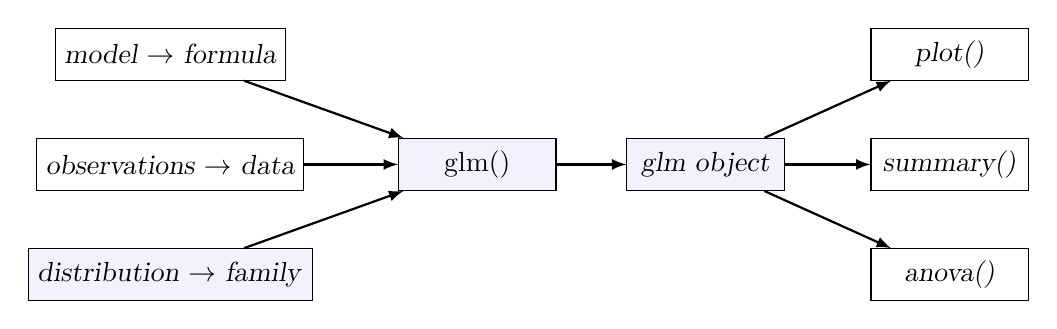
\begin{tikzpicture}[node distance=1.4cm, scale=0.5]
\node (model) [tprocess] {\textsl{model $\to$ \code{formula}}};
\node (data) [tprocess, below of=model] {\textsl{observations $\to$ \code{data}}};
\node (family) [tprocess, below of=data, fill=blue!5] {\textsl{distribution $\to$ \code{family}}};
\node (fitfun) [tprocess, right of=data, xshift=2.5cm, fill=blue!5] {\code{glm()}};
\node (fm) [tprocess, color = black, right of=fitfun, xshift=1.5cm, fill=blue!5] {\textsl{\code{glm} object}};
\node (summary) [tprocess, color = black, right of=fm, xshift=1.7cm] {\textsl{\code{summary()}}};
\node (anova) [tprocess, color = black, below of=summary] {\textsl{\code{anova()}}};
\node (plot) [tprocess, color = black, above of=summary] {\textsl{\code{plot()}}};
\draw [arrow] (model) -- (fitfun);
\draw [arrow] (data) -- (fitfun);
\draw [arrow] (family) -- (fitfun);
\draw [arrow] (fitfun) -- (fm);
\draw [arrow] (fm) -- (plot);
\draw [arrow] (fm) -- (anova);
\draw [arrow] (fm) -- (summary);
\end{tikzpicture}
\end{small}
\end{center}

For the analysis of the \Rdata{InsectSpray} data set above (section \ref{sec:anova} on page \pageref{sec:anova}), the Normal distribution is not a good approximation as count data deviates from it. This was visible in the quantile--quantile plot above.

For count data, GLMs provide a better alternative. In the example below we fit the same model as above, but we assume a quasi-Poisson distribution instead of the Normal. In addition to the model formula we need to pass an argument through \code{family} giving the error distribution to be assumed---the default for \code{family} is \code{gaussian} or Normal distribution.

\begin{knitrout}\footnotesize
\definecolor{shadecolor}{rgb}{0.969, 0.969, 0.969}\color{fgcolor}\begin{kframe}
\begin{alltt}
\hlstd{fm10} \hlkwb{<-} \hlkwd{glm}\hlstd{(count} \hlopt{~} \hlstd{spray,} \hlkwc{data} \hlstd{= InsectSprays,} \hlkwc{family} \hlstd{= quasipoisson)}
\hlkwd{anova}\hlstd{(fm10)}
\end{alltt}
\begin{verbatim}
## Analysis of Deviance Table
## 
## Model: quasipoisson, link: log
## 
## Response: count
## 
## Terms added sequentially (first to last)
## 
## 
##       Df Deviance Resid. Df Resid. Dev
## NULL                     71     409.04
## spray  5   310.71        66      98.33
\end{verbatim}
\end{kframe}
\end{knitrout}

The printout from the \Rfunction{anova()} method for GLM fits has some differences to that for LM fits. By default, no significance test is computed, as a knowledgeable choice is required depending on the characteristics of the model and data. We here use \code{"F"} as an argument to request an $F$-test.

\begin{knitrout}\footnotesize
\definecolor{shadecolor}{rgb}{0.969, 0.969, 0.969}\color{fgcolor}\begin{kframe}
\begin{alltt}
\hlkwd{anova}\hlstd{(fm10,} \hlkwc{test} \hlstd{=} \hlstr{"F"}\hlstd{)}
\end{alltt}
\begin{verbatim}
## Analysis of Deviance Table
## 
## Model: quasipoisson, link: log
## 
## Response: count
## 
## Terms added sequentially (first to last)
## 
## 
##       Df Deviance Resid. Df Resid. Dev      F    Pr(>F)    
## NULL                     71     409.04                     
## spray  5   310.71        66      98.33 41.216 < 2.2e-16 ***
## ---
## Signif. codes:  0 '***' 0.001 '**' 0.01 '*' 0.05 '.' 0.1 ' ' 1
\end{verbatim}
\end{kframe}
\end{knitrout}

Method \Rfunction{plot()} as for linear-model fits, produces diagnosis plots. We show as above the q-q-plot of residuals.

\begin{knitrout}\footnotesize
\definecolor{shadecolor}{rgb}{0.969, 0.969, 0.969}\color{fgcolor}\begin{kframe}
\begin{alltt}
\hlkwd{plot}\hlstd{(fm10,} \hlkwc{which} \hlstd{=} \hlnum{3}\hlstd{)}
\end{alltt}
\end{kframe}

{\centering 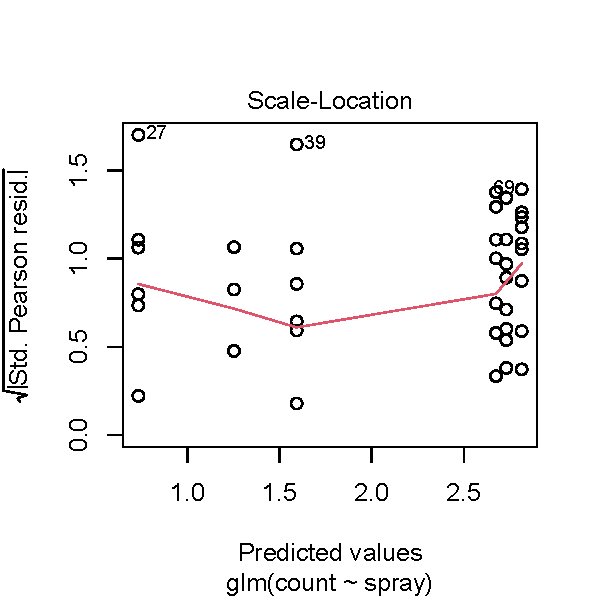
\includegraphics[width=.54\textwidth]{figure/pos-model-11-1} 

}


\end{knitrout}

We can extract different components similarly as described for linear models (see section \ref{sec:stat:LM} on page \pageref{sec:stat:LM}).

\begin{knitrout}\footnotesize
\definecolor{shadecolor}{rgb}{0.969, 0.969, 0.969}\color{fgcolor}\begin{kframe}
\begin{alltt}
\hlkwd{class}\hlstd{(fm10)}
\end{alltt}
\begin{verbatim}
## [1] "glm" "lm"
\end{verbatim}
\begin{alltt}
\hlkwd{summary}\hlstd{(fm10)}
\end{alltt}
\begin{verbatim}
## 
## Call:
## glm(formula = count ~ spray, family = quasipoisson, data = InsectSprays)
## 
## Deviance Residuals: 
##     Min       1Q   Median       3Q      Max  
## -2.3852  -0.8876  -0.1482   0.6063   2.6922  
## 
## Coefficients:
##             Estimate Std. Error t value Pr(>|t|)    
## (Intercept)  2.67415    0.09309  28.728  < 2e-16 ***
## sprayB       0.05588    0.12984   0.430    0.668    
## sprayC      -1.94018    0.26263  -7.388 3.30e-10 ***
## sprayD      -1.08152    0.18499  -5.847 1.70e-07 ***
## sprayE      -1.42139    0.21110  -6.733 4.82e-09 ***
## sprayF       0.13926    0.12729   1.094    0.278    
## ---
## Signif. codes:  0 '***' 0.001 '**' 0.01 '*' 0.05 '.' 0.1 ' ' 1
## 
## (Dispersion parameter for quasipoisson family taken to be 1.507713)
## 
##     Null deviance: 409.041  on 71  degrees of freedom
## Residual deviance:  98.329  on 66  degrees of freedom
## AIC: NA
## 
## Number of Fisher Scoring iterations: 5
\end{verbatim}
\begin{alltt}
\hlkwd{head}\hlstd{(}\hlkwd{residuals}\hlstd{(fm10))}
\end{alltt}
\begin{verbatim}
##          1          2          3          4          5          6 
## -1.2524891 -2.1919537  1.3650439 -0.1320721 -0.1320721 -0.6768988
\end{verbatim}
\begin{alltt}
\hlkwd{head}\hlstd{(}\hlkwd{fitted}\hlstd{(fm10))}
\end{alltt}
\begin{verbatim}
##    1    2    3    4    5    6 
## 14.5 14.5 14.5 14.5 14.5 14.5
\end{verbatim}
\end{kframe}
\end{knitrout}

\begin{explainbox}
If we use \code{str()} or \code{names()} we can see that there are some differences with respect to linear model fits. The returned object is of a different class and contains some members not present in linear models. Two of these have to do with the iterative approximation method used, \code{iter} contains the number of iterations used  and \code{converged} the success or not in finding a solution.

\begin{knitrout}\footnotesize
\definecolor{shadecolor}{rgb}{0.969, 0.969, 0.969}\color{fgcolor}\begin{kframe}
\begin{alltt}
\hlkwd{names}\hlstd{(fm10)}
\end{alltt}
\begin{verbatim}
##  [1] "coefficients"      "residuals"         "fitted.values"    
##  [4] "effects"           "R"                 "rank"             
##  [7] "qr"                "family"            "linear.predictors"
## [10] "deviance"          "aic"               "null.deviance"    
## [13] "iter"              "weights"           "prior.weights"    
## [16] "df.residual"       "df.null"           "y"                
## [19] "converged"         "boundary"          "model"            
## [22] "call"              "formula"           "terms"            
## [25] "data"              "offset"            "control"          
## [28] "method"            "contrasts"         "xlevels"
\end{verbatim}
\begin{alltt}
\hlstd{fm10}\hlopt{$}\hlstd{converged}
\end{alltt}
\begin{verbatim}
## [1] TRUE
\end{verbatim}
\begin{alltt}
\hlstd{fm10}\hlopt{$}\hlstd{iter}
\end{alltt}
\begin{verbatim}
## [1] 5
\end{verbatim}
\end{kframe}
\end{knitrout}
\end{explainbox}

\index{generalized linear models|)}

\section{Non-linear regression}\label{sec:stat:NLS}
\index{non-linear models|(}%
\index{models!non-linear|see{non-linear models}}%
\index{NLS|see{non-linear models}}

Function \Rfunction{nls()} is \Rlang's workhorse for fitting non-linear models. By \emph{non-linear} it is meant non-linear \emph{in the parameters} whose values are being estimated through fitting the model to data. This is different from the shape of the function when plotted---i.e., polynomials of any degree are linear models. In contrast, the Michaelis-Menten equation used in chemistry and the Gompertz equation used to describe growth are non-linear models in their parameters.

While analytical algorithms exist for finding estimates for the parameters of linear models, in the case of non-linear models, the estimates are obtained by approximation. For analytical solutions, estimates can always be obtained, except in infrequent pathological cases where reliance on floating point numbers with limited resolution introduces rounding errors that ``break'' mathematical algorithms that are valid for real numbers. For approximations obtained through iteration, cases when the algorithm fails to \emph{converge} onto an answer are relatively common. Iterative algorithms attempt to improve an initial guess for the values of the parameters to be estimated, a guess frequently supplied by the user. In each iteration the estimate obtained in the previous iteration is used as the starting value, and this process is repeated one time after another. The expectation is that after a finite number of iterations the algorithm will converge into a solution that ``cannot'' be improved further. In real life we stop iteration when the improvement in the fit is smaller than a certain threshold, or when no convergence has been achieved after a certain maximum number of iterations. In the first case, we usually obtain good estimates; in the second case, we do not obtain usable estimates and need to look for different ways of obtaining them. When convergence fails, the first thing to do is to try different starting values and if this also fails, switch to a different computational algorithm. These steps usually help, but not always. Good starting values are in many cases crucial and in some cases ``guesses'' can be obtained using either graphical or analytical approximations.

\begin{center}
\begin{small}
\begin{tikzpicture}[node distance=1.4cm, scale=0.5]
\node (model) [tprocess] {\textsl{model $\to$ \code{formula}}};
\node (data) [tprocess, below of=model] {\textsl{observations $\to$ \code{data}}};
\node (guess) [tprocess, below of=data, fill=blue!5] {\textsl{guesses $\to$ \code{start}}};
\node (fitfun) [tprocess, right of=data, xshift=2.5cm, fill=blue!5] {\code{nls()}};
\node (fm) [tprocess, color = black, right of=fitfun, xshift=1.5cm, fill=blue!5] {\textsl{\code{nls} object}};
\node (summary) [tprocess, color = black, right of=fm, xshift=1.7cm] {\textsl{\code{summary()}}};
\node (anova) [tprocess, color = black, below of=summary] {\textsl{\code{anova()}}};
\node (plot) [tprocess, color = black, above of=summary] {\textsl{\code{plot()}}};
\draw [arrow] (model) -- (fitfun);
\draw [arrow] (data) -- (fitfun);
\draw [arrow] (family) -- (fitfun);
\draw [arrow] (fitfun) -- (fm);
\draw [arrow] (fm) -- (plot);
\draw [arrow] (fm) -- (anova);
\draw [arrow] (fm) -- (summary);
\end{tikzpicture}
\end{small}
\end{center}

For functions for which computational algorithms exist for ``guessing'' suitable starting values, \Rlang provides a mechanism for packaging the function to be fitted together with the function generating the starting values. These functions go by the name of \emph{self-starting functions} and relieve the user from the burden of guessing and supplying suitable starting values. The\index{self-starting functions} self-starting functions available in \Rlang are \code{SSasymp()}, \code{SSasympOff()}, \code{SSasympOrig()}, \code{SSbiexp()}, \code{SSfol()}, \code{SSfpl()}, \code{SSgompertz()}, \code{SSlogis()}, \code{SSmicmen()}, and \code{SSweibull()}. Function \code{selfStart()} can be used to define new ones. All these functions can be used when fitting models with \Rfunction{nls} or \Rfunction{nlme}. Please, check the respective help pages for details.

In the case of \Rfunction{nls()} the specification of the model to be fitted differs from that used for linear models. We will use as an example fitting the Michaelis-Menten equation\index{Michaelis-Menten equation} describing reaction kinetics\index{chemical reaction kinetics} in biochemistry and chemistry. The mathematical formulation is given by:

\begin{equation}\label{eq:michaelis:menten}
v = \frac{\mathrm{d} [P]}{\mathrm{d} t} = \frac{V_{\mathrm{max}} [S]}{K_{\mathrm{M}} + [S]}
\end{equation}

The function takes its name from Michaelis and Menten's paper from 1913 \autocite{Johnson2011}. A self-starting function implementing the Michaelis-Menten equation is available in \Rlang under the name \Rfunction{SSmicmen()}\index{models!selfstart@{\texttt{selfStart}}}. We will use the \Rdata{Puromycin} data set.

\begin{knitrout}\footnotesize
\definecolor{shadecolor}{rgb}{0.969, 0.969, 0.969}\color{fgcolor}\begin{kframe}
\begin{alltt}
\hlkwd{data}\hlstd{(Puromycin)}
\hlkwd{names}\hlstd{(Puromycin)}
\end{alltt}
\begin{verbatim}
## [1] "conc"  "rate"  "state"
\end{verbatim}
\end{kframe}
\end{knitrout}

\begin{knitrout}\footnotesize
\definecolor{shadecolor}{rgb}{0.969, 0.969, 0.969}\color{fgcolor}\begin{kframe}
\begin{alltt}
\hlstd{fm21} \hlkwb{<-} \hlkwd{nls}\hlstd{(rate} \hlopt{~} \hlkwd{SSmicmen}\hlstd{(conc, Vm, K),} \hlkwc{data} \hlstd{= Puromycin,}
            \hlkwc{subset} \hlstd{= state} \hlopt{==} \hlstr{"treated"}\hlstd{)}
\end{alltt}
\end{kframe}
\end{knitrout}

We can extract different components similarly as described for linear models (see section \ref{sec:stat:LM} on page \pageref{sec:stat:LM}).

\begin{knitrout}\footnotesize
\definecolor{shadecolor}{rgb}{0.969, 0.969, 0.969}\color{fgcolor}\begin{kframe}
\begin{alltt}
\hlkwd{class}\hlstd{(fm21)}
\end{alltt}
\begin{verbatim}
## [1] "nls"
\end{verbatim}
\begin{alltt}
\hlkwd{summary}\hlstd{(fm21)}
\end{alltt}
\begin{verbatim}
## 
## Formula: rate ~ SSmicmen(conc, Vm, K)
## 
## Parameters:
##     Estimate Std. Error t value Pr(>|t|)    
## Vm 2.127e+02  6.947e+00  30.615 3.24e-11 ***
## K  6.412e-02  8.281e-03   7.743 1.57e-05 ***
## ---
## Signif. codes:  0 '***' 0.001 '**' 0.01 '*' 0.05 '.' 0.1 ' ' 1
## 
## Residual standard error: 10.93 on 10 degrees of freedom
## 
## Number of iterations to convergence: 0 
## Achieved convergence tolerance: 1.937e-06
\end{verbatim}
\begin{alltt}
\hlkwd{residuals}\hlstd{(fm21)}
\end{alltt}
\begin{verbatim}
##  [1]  25.4339970  -3.5660030  -5.8109606   4.1890394 -11.3616076   4.6383924
##  [7]  -5.6846886 -12.6846886   0.1670799  10.1670799   6.0311724  -0.9688276
## attr(,"label")
## [1] "Residuals"
\end{verbatim}
\begin{alltt}
\hlkwd{fitted}\hlstd{(fm21)}
\end{alltt}
\begin{verbatim}
##  [1]  50.5660  50.5660 102.8110 102.8110 134.3616 134.3616 164.6847 164.6847
##  [9] 190.8329 190.8329 200.9688 200.9688
## attr(,"label")
## [1] "Fitted values"
\end{verbatim}
\end{kframe}
\end{knitrout}

\begin{explainbox}
If we use \code{str()} or \code{names()} we can see that there are differences with respect to linear model and generalized model fits. The returned object is of class \code{nls} and contains some new members and lacks others. Two members are related to the iterative approximation method used, \code{control} containing nested members holding iteration settings, and \code{convInfo} (convergence information) with nested members with information on the outcome of the iterative algorithm.

\begin{knitrout}\footnotesize
\definecolor{shadecolor}{rgb}{0.969, 0.969, 0.969}\color{fgcolor}\begin{kframe}
\begin{alltt}
\hlkwd{str}\hlstd{(fm21,} \hlkwc{max.level} \hlstd{=} \hlnum{1}\hlstd{)}
\end{alltt}
\begin{verbatim}
## List of 6
##  $ m          :List of 16
##   ..- attr(*, "class")= chr "nlsModel"
##  $ convInfo   :List of 5
##  $ data       : symbol Puromycin
##  $ call       : language nls(formula = rate ~ SSmicmen(conc, Vm, K), data = Puromycin, subset = state ==      "treated", algorithm = "defa| __truncated__ ...
##  $ dataClasses: Named chr "numeric"
##   ..- attr(*, "names")= chr "conc"
##  $ control    :List of 7
##  - attr(*, "class")= chr "nls"
\end{verbatim}
\end{kframe}
\end{knitrout}

\begin{knitrout}\footnotesize
\definecolor{shadecolor}{rgb}{0.969, 0.969, 0.969}\color{fgcolor}\begin{kframe}
\begin{alltt}
\hlstd{fm21}\hlopt{$}\hlstd{convInfo}
\end{alltt}
\begin{verbatim}
## $isConv
## [1] TRUE
## 
## $finIter
## [1] 0
## 
## $finTol
## [1] 1.937028e-06
## 
## $stopCode
## [1] 0
## 
## $stopMessage
## [1] "converged"
\end{verbatim}
\end{kframe}
\end{knitrout}
\end{explainbox}

\index{non-linear models|)}

\section{Model formulas}\label{sec:stat:formulas}
\index{model formulas|(}
\Rlang is consistent in how it treats various objects, to a extent that can be surprising to those familiar with other computer languages. Model formulas are objects of class \Rclass{formula} and mode \Rclass{call} and can be manipulated and stored similarly to objects of other classes.

\begin{knitrout}\footnotesize
\definecolor{shadecolor}{rgb}{0.969, 0.969, 0.969}\color{fgcolor}\begin{kframe}
\begin{alltt}
\hlkwd{class}\hlstd{(y} \hlopt{~} \hlstd{x)}
\end{alltt}
\begin{verbatim}
## [1] "formula"
\end{verbatim}
\begin{alltt}
\hlkwd{mode}\hlstd{(y} \hlopt{~} \hlstd{x)}
\end{alltt}
\begin{verbatim}
## [1] "call"
\end{verbatim}
\end{kframe}
\end{knitrout}

Like any other \Rlang object formulas can be assigned to variables and be members of lists and vectors. Consequently, the first linear model fit example from page \pageref{chunk:lm:models1} can be rewritten as follows.

\begin{knitrout}\footnotesize
\definecolor{shadecolor}{rgb}{0.969, 0.969, 0.969}\color{fgcolor}\begin{kframe}
\begin{alltt}
\hlstd{my.formula} \hlkwb{<-} \hlstd{dist} \hlopt{~} \hlnum{1} \hlopt{+} \hlstd{speed}
\hlstd{fm1} \hlkwb{<-} \hlkwd{lm}\hlstd{(my.formula,} \hlkwc{data}\hlstd{=cars)}
\end{alltt}
\end{kframe}
\end{knitrout}

In some situations models lacking a lhs term (a term on the left hand side of \verb|~|) are used but at least one term on the must be present in the rhs.
\begin{knitrout}\footnotesize
\definecolor{shadecolor}{rgb}{0.969, 0.969, 0.969}\color{fgcolor}\begin{kframe}
\begin{alltt}
\hlkwd{class}\hlstd{(}\hlopt{~} \hlstd{x} \hlopt{+} \hlstd{y)}
\end{alltt}
\begin{verbatim}
## [1] "formula"
\end{verbatim}
\begin{alltt}
\hlkwd{mode}\hlstd{(}\hlopt{~} \hlstd{x} \hlopt{+} \hlstd{y)}
\end{alltt}
\begin{verbatim}
## [1] "call"
\end{verbatim}
\begin{alltt}
\hlkwd{is.empty.model}\hlstd{(}\hlopt{~} \hlstd{x} \hlopt{+} \hlstd{y)}
\end{alltt}
\begin{verbatim}
## [1] FALSE
\end{verbatim}
\end{kframe}
\end{knitrout}

\begin{explainbox}
In this box we highlight, for completeness, some idiosyncracies of \Rlang formulas that are seldom important in everyday use but can be important in advanced scripts. As with other classes, empty objects or vectors of length zero are valid. In the case of formulas there is an additional kind of emptiness, a formula describing a model with no explanatory terms on its rhs.

An empty object of class \Rclass{formula} can be created with \code{formula()}. The last statement triggers an error as there is no model formula.

\begin{knitrout}\footnotesize
\definecolor{shadecolor}{rgb}{0.969, 0.969, 0.969}\color{fgcolor}\begin{kframe}
\begin{alltt}
\hlkwd{class}\hlstd{(}\hlkwd{formula}\hlstd{())}
\end{alltt}
\begin{verbatim}
## [1] "formula"
\end{verbatim}
\begin{alltt}
\hlkwd{mode}\hlstd{(}\hlkwd{formula}\hlstd{())}
\end{alltt}
\begin{verbatim}
## [1] "list"
\end{verbatim}
\begin{alltt}
\hlcom{# is.empty.model(formula())}
\end{alltt}
\end{kframe}
\end{knitrout}

An object of class \Rclass{formula} containing a formula object describing an empty model. While \verb|y ~ 1| describes a model with only an intercept (estimating $a = \bar{x}$), \verb|y ~ 0| or its equivalent \verb|y ~ -1|, describes an empty model that cannot be fitted to data.

\begin{knitrout}\footnotesize
\definecolor{shadecolor}{rgb}{0.969, 0.969, 0.969}\color{fgcolor}\begin{kframe}
\begin{alltt}
\hlkwd{class}\hlstd{(y} \hlopt{~} \hlnum{0}\hlstd{)}
\end{alltt}
\begin{verbatim}
## [1] "formula"
\end{verbatim}
\begin{alltt}
\hlkwd{mode}\hlstd{(y} \hlopt{~} \hlnum{0}\hlstd{)}
\end{alltt}
\begin{verbatim}
## [1] "call"
\end{verbatim}
\begin{alltt}
\hlkwd{is.empty.model}\hlstd{(y} \hlopt{~} \hlnum{0}\hlstd{)}
\end{alltt}
\begin{verbatim}
## [1] TRUE
\end{verbatim}
\begin{alltt}
\hlkwd{is.empty.model}\hlstd{(y} \hlopt{~} \hlnum{1}\hlstd{)}
\end{alltt}
\begin{verbatim}
## [1] FALSE
\end{verbatim}
\begin{alltt}
\hlkwd{is.empty.model}\hlstd{(y} \hlopt{~} \hlstd{x)}
\end{alltt}
\begin{verbatim}
## [1] FALSE
\end{verbatim}
\end{kframe}
\end{knitrout}

The value returned by \Rmethod{length()} on a single formula is not always 1, the number of formulas in the vector of formulas, but instead the number of components in the formula. For longer and shorter vectors, it does return the number of member formulae. Because of this, it is better to store model formulas in objects of class \Rclass{list} than in vectors, as \Rfunction{length()} consistently returns the expected value on lists.

\begin{knitrout}\footnotesize
\definecolor{shadecolor}{rgb}{0.969, 0.969, 0.969}\color{fgcolor}\begin{kframe}
\begin{alltt}
\hlkwd{length}\hlstd{(}\hlkwd{formula}\hlstd{())}
\end{alltt}
\begin{verbatim}
## [1] 0
\end{verbatim}
\begin{alltt}
\hlkwd{length}\hlstd{(y} \hlopt{~} \hlnum{0}\hlstd{)}
\end{alltt}
\begin{verbatim}
## [1] 3
\end{verbatim}
\begin{alltt}
\hlkwd{length}\hlstd{(y} \hlopt{~} \hlnum{1}\hlstd{)}
\end{alltt}
\begin{verbatim}
## [1] 3
\end{verbatim}
\begin{alltt}
\hlkwd{length}\hlstd{(y} \hlopt{~} \hlstd{x)}
\end{alltt}
\begin{verbatim}
## [1] 3
\end{verbatim}
\begin{alltt}
\hlkwd{length}\hlstd{(}\hlkwd{c}\hlstd{(y} \hlopt{~} \hlnum{1}\hlstd{, y} \hlopt{~} \hlstd{x))}
\end{alltt}
\begin{verbatim}
## [1] 2
\end{verbatim}
\begin{alltt}
\hlkwd{length}\hlstd{(}\hlkwd{list}\hlstd{(y} \hlopt{~} \hlnum{1}\hlstd{))}
\end{alltt}
\begin{verbatim}
## [1] 1
\end{verbatim}
\begin{alltt}
\hlkwd{length}\hlstd{(}\hlkwd{list}\hlstd{(y} \hlopt{~} \hlnum{1}\hlstd{, y} \hlopt{~} \hlstd{x))}
\end{alltt}
\begin{verbatim}
## [1] 2
\end{verbatim}
\end{kframe}
\end{knitrout}

\end{explainbox}

In the examples in previous sections we fitted simple models. More complex ones can be easily formulated using the same syntax. First of all, one can avoid use of operator \code{*} and explicitly define all individual main effects and interactions using operators \code{+} and \code{:}. The syntax implemented in base \Rlang allows grouping by means of parentheses, so it is also possible to exclude some interactions by combining the use of \code{*} and parentheses.

The same symbols as for arithmetic operators are used for model formulas. Within a formula, symbols are interpreted according to formula syntax. When we mean an arithmetic operation that could be interpreted as being part of the model formula we need to ``protect'' it by means of the identity function \Rfunction{I()}. The next two examples define formulas for models with only one explanatory variable. With formulas like these, the explanatory variable will be computed on the fly when fitting the model to data. In the first case below we need to explicitly protect the addition of the two variables into their sum, because otherwise they would be interpreted as two separate explanatory variables in the model. In the second case, \Rfunction{log()} cannot be interpreted as part of the model formula, and consequently does not require additional protection, neither does the expression passed as its argument.

\begin{knitrout}\footnotesize
\definecolor{shadecolor}{rgb}{0.969, 0.969, 0.969}\color{fgcolor}\begin{kframe}
\begin{alltt}
\hlstd{y} \hlopt{~} \hlkwd{I}\hlstd{(x1} \hlopt{+} \hlstd{x2)}
\hlstd{y} \hlopt{~} \hlkwd{log}\hlstd{(x1} \hlopt{+} \hlstd{x2)}
\end{alltt}
\end{kframe}
\end{knitrout}

\Rlang formula syntax allows alternative ways for specifying interaction terms. They allow ``abbreviated'' ways of entering formulas, which for complex experimental designs saves typing and can improve clarity. As seen above, operator \code{*} saves us from having to explicitly indicate all the interaction terms in a full factorial model.

\begin{knitrout}\footnotesize
\definecolor{shadecolor}{rgb}{0.969, 0.969, 0.969}\color{fgcolor}\begin{kframe}
\begin{alltt}
\hlstd{y} \hlopt{~} \hlstd{x1} \hlopt{+} \hlstd{x2} \hlopt{+} \hlstd{x3} \hlopt{+} \hlstd{x1}\hlopt{:}\hlstd{x2} \hlopt{+} \hlstd{x1}\hlopt{:}\hlstd{x3} \hlopt{+} \hlstd{x2}\hlopt{:}\hlstd{x3} \hlopt{+} \hlstd{x1}\hlopt{:}\hlstd{x2}\hlopt{:}\hlstd{x3}
\end{alltt}
\end{kframe}
\end{knitrout}

Can be replaced by a concise equivalent.

\begin{knitrout}\footnotesize
\definecolor{shadecolor}{rgb}{0.969, 0.969, 0.969}\color{fgcolor}\begin{kframe}
\begin{alltt}
\hlstd{y} \hlopt{~} \hlstd{x1} \hlopt{*} \hlstd{x2} \hlopt{*} \hlstd{x3}
\end{alltt}
\end{kframe}
\end{knitrout}

When the model to be specified does not include all possible interaction terms, we can combine the concise notation with parentheses.

\begin{knitrout}\footnotesize
\definecolor{shadecolor}{rgb}{0.969, 0.969, 0.969}\color{fgcolor}\begin{kframe}
\begin{alltt}
\hlstd{y} \hlopt{~} \hlstd{x1} \hlopt{+} \hlstd{(x2} \hlopt{*} \hlstd{x3)}
\hlstd{y} \hlopt{~} \hlstd{x1} \hlopt{+} \hlstd{x2} \hlopt{+} \hlstd{x3} \hlopt{+} \hlstd{x2}\hlopt{:}\hlstd{x3}
\end{alltt}
\end{kframe}
\end{knitrout}

That the two model formulas above are equivalent, can be seen using \code{terms()}

\begin{knitrout}\footnotesize
\definecolor{shadecolor}{rgb}{0.969, 0.969, 0.969}\color{fgcolor}\begin{kframe}
\begin{alltt}
\hlkwd{terms}\hlstd{(y} \hlopt{~} \hlstd{x1} \hlopt{+} \hlstd{(x2} \hlopt{*} \hlstd{x3))}
\end{alltt}
\begin{verbatim}
## y ~ x1 + (x2 * x3)
## attr(,"variables")
## list(y, x1, x2, x3)
## attr(,"factors")
##    x1 x2 x3 x2:x3
## y   0  0  0     0
## x1  1  0  0     0
## x2  0  1  0     1
## x3  0  0  1     1
## attr(,"term.labels")
## [1] "x1"    "x2"    "x3"    "x2:x3"
## attr(,"order")
## [1] 1 1 1 2
## attr(,"intercept")
## [1] 1
## attr(,"response")
## [1] 1
## attr(,".Environment")
## <environment: R_GlobalEnv>
\end{verbatim}
\end{kframe}
\end{knitrout}

\begin{knitrout}\footnotesize
\definecolor{shadecolor}{rgb}{0.969, 0.969, 0.969}\color{fgcolor}\begin{kframe}
\begin{alltt}
\hlstd{y} \hlopt{~} \hlstd{x1} \hlopt{*} \hlstd{(x2} \hlopt{+} \hlstd{x3)}
\hlstd{y} \hlopt{~} \hlstd{x1} \hlopt{+} \hlstd{x2} \hlopt{+} \hlstd{x3} \hlopt{+} \hlstd{x1}\hlopt{:}\hlstd{x2} \hlopt{+} \hlstd{x1}\hlopt{:}\hlstd{x3}
\end{alltt}
\end{kframe}
\end{knitrout}

\begin{knitrout}\footnotesize
\definecolor{shadecolor}{rgb}{0.969, 0.969, 0.969}\color{fgcolor}\begin{kframe}
\begin{alltt}
\hlkwd{terms}\hlstd{(y} \hlopt{~} \hlstd{x1} \hlopt{*} \hlstd{(x2} \hlopt{+} \hlstd{x3))}
\end{alltt}
\begin{verbatim}
## y ~ x1 * (x2 + x3)
## attr(,"variables")
## list(y, x1, x2, x3)
## attr(,"factors")
##    x1 x2 x3 x1:x2 x1:x3
## y   0  0  0     0     0
## x1  1  0  0     1     1
## x2  0  1  0     1     0
## x3  0  0  1     0     1
## attr(,"term.labels")
## [1] "x1"    "x2"    "x3"    "x1:x2" "x1:x3"
## attr(,"order")
## [1] 1 1 1 2 2
## attr(,"intercept")
## [1] 1
## attr(,"response")
## [1] 1
## attr(,".Environment")
## <environment: R_GlobalEnv>
\end{verbatim}
\end{kframe}
\end{knitrout}

The \code{\textasciicircum{}} operator provides a concise notation to limit the order of the interaction terms included in a formula.

\begin{knitrout}\footnotesize
\definecolor{shadecolor}{rgb}{0.969, 0.969, 0.969}\color{fgcolor}\begin{kframe}
\begin{alltt}
\hlstd{y} \hlopt{~} \hlstd{(x1} \hlopt{+} \hlstd{x2} \hlopt{+} \hlstd{x3)}\hlopt{^}\hlnum{2}
\hlstd{y} \hlopt{~} \hlstd{x1} \hlopt{+} \hlstd{x2} \hlopt{+} \hlstd{x3} \hlopt{+} \hlstd{x1}\hlopt{:}\hlstd{x2} \hlopt{+} \hlstd{x1}\hlopt{:}\hlstd{x3} \hlopt{+} \hlstd{x2}\hlopt{:}\hlstd{x3}
\end{alltt}
\end{kframe}
\end{knitrout}

\begin{knitrout}\footnotesize
\definecolor{shadecolor}{rgb}{0.969, 0.969, 0.969}\color{fgcolor}\begin{kframe}
\begin{alltt}
\hlkwd{terms}\hlstd{(y} \hlopt{~} \hlstd{(x1} \hlopt{+} \hlstd{x2} \hlopt{+} \hlstd{x3)}\hlopt{^}\hlnum{2}\hlstd{)}
\end{alltt}
\begin{verbatim}
## y ~ (x1 + x2 + x3)^2
## attr(,"variables")
## list(y, x1, x2, x3)
## attr(,"factors")
##    x1 x2 x3 x1:x2 x1:x3 x2:x3
## y   0  0  0     0     0     0
## x1  1  0  0     1     1     0
## x2  0  1  0     1     0     1
## x3  0  0  1     0     1     1
## attr(,"term.labels")
## [1] "x1"    "x2"    "x3"    "x1:x2" "x1:x3" "x2:x3"
## attr(,"order")
## [1] 1 1 1 2 2 2
## attr(,"intercept")
## [1] 1
## attr(,"response")
## [1] 1
## attr(,".Environment")
## <environment: R_GlobalEnv>
\end{verbatim}
\end{kframe}
\end{knitrout}

\begin{advplayground}
For operator \code{\textasciicircum{}} to behave as expected, its first operand should be a formula with no interactions!  Compare the result of expanding these two formulas with \Rfunction{terms()}.

\begin{knitrout}\footnotesize
\definecolor{shadecolor}{rgb}{0.969, 0.969, 0.969}\color{fgcolor}\begin{kframe}
\begin{alltt}
\hlstd{y} \hlopt{~} \hlstd{(x1} \hlopt{+} \hlstd{x2} \hlopt{+} \hlstd{x3)}\hlopt{^}\hlnum{2}
\hlstd{y} \hlopt{~} \hlstd{(x1} \hlopt{*} \hlstd{x2} \hlopt{*} \hlstd{x3)}\hlopt{^}\hlnum{2}
\end{alltt}
\end{kframe}
\end{knitrout}

\end{advplayground}

Operator \code{\%in\%} can also be used as a shortcut for including only some of all the possible interaction terms in a formula.

\begin{knitrout}\footnotesize
\definecolor{shadecolor}{rgb}{0.969, 0.969, 0.969}\color{fgcolor}\begin{kframe}
\begin{alltt}
\hlstd{y} \hlopt{~} \hlstd{x1} \hlopt{+} \hlstd{x2} \hlopt{+} \hlstd{x1} \hlopt \hlstd{x2}
\end{alltt}
\end{kframe}
\end{knitrout}

\begin{knitrout}\footnotesize
\definecolor{shadecolor}{rgb}{0.969, 0.969, 0.969}\color{fgcolor}\begin{kframe}
\begin{alltt}
\hlkwd{terms}\hlstd{(y} \hlopt{~} \hlstd{x1} \hlopt{+} \hlstd{x2} \hlopt{+} \hlstd{x1} \hlopt \hlstd{x2)}
\end{alltt}
\begin{verbatim}
## y ~ x1 + x2 + x1 %in% x2
## attr(,"variables")
## list(y, x1, x2)
## attr(,"factors")
##    x1 x2 x1:x2
## y   0  0     0
## x1  1  0     1
## x2  0  1     1
## attr(,"term.labels")
## [1] "x1"    "x2"    "x1:x2"
## attr(,"order")
## [1] 1 1 2
## attr(,"intercept")
## [1] 1
## attr(,"response")
## [1] 1
## attr(,".Environment")
## <environment: R_GlobalEnv>
\end{verbatim}
\end{kframe}
\end{knitrout}

\begin{playground}
Execute the examples below using the \Rdata{npk} data set from \Rlang. They demonstrate the use of different model formulas in ANOVA\index{analysis of variance!model formula}. Use these examples plus your own variations on the same theme to build your understanding of the syntax of model formulas. Based on the terms displayed in the ANOVA tables, first work out what models are being fitted in each case. In a second step, write each of the models using a mathematical formulation. Finally, think how model choice may affect the conclusions from an analysis of variance.

% runs fine but crashes LaTeX
\begin{knitrout}\footnotesize
\definecolor{shadecolor}{rgb}{0.969, 0.969, 0.969}\color{fgcolor}\begin{kframe}
\begin{alltt}
\hlkwd{data}\hlstd{(npk)}
\hlkwd{anova}\hlstd{(}\hlkwd{lm}\hlstd{(yield} \hlopt{~} \hlstd{N} \hlopt{*} \hlstd{P} \hlopt{*} \hlstd{K,} \hlkwc{data} \hlstd{= npk))}
\hlkwd{anova}\hlstd{(}\hlkwd{lm}\hlstd{(yield} \hlopt{~} \hlstd{(N} \hlopt{+} \hlstd{P} \hlopt{+} \hlstd{K)}\hlopt{^}\hlnum{2}\hlstd{,} \hlkwc{data} \hlstd{= npk))}
\hlkwd{anova}\hlstd{(}\hlkwd{lm}\hlstd{(yield} \hlopt{~} \hlstd{N} \hlopt{+} \hlstd{P} \hlopt{+} \hlstd{K} \hlopt{+} \hlstd{P} \hlopt \hlstd{N} \hlopt{+} \hlstd{K} \hlopt \hlstd{N,} \hlkwc{data} \hlstd{= npk))}
\hlkwd{anova}\hlstd{(}\hlkwd{lm}\hlstd{(yield} \hlopt{~} \hlstd{N} \hlopt{+} \hlstd{P} \hlopt{+} \hlstd{K} \hlopt{+} \hlstd{N} \hlopt \hlstd{P} \hlopt{+} \hlstd{K} \hlopt \hlstd{P,} \hlkwc{data} \hlstd{= npk))}
\end{alltt}
\end{kframe}
\end{knitrout}

\end{playground}

Nesting of factors in experiments using hierarchical designs such as split-plots or repeated measures, results in the need to compute additional error terms, differing in their degrees of freedom. In such a design, different effects are tested based on different error terms. Whether nesting exists or not is a property of an experiment. It is decided as part of the design of the experiment based on the mechanics of treatment assignment to experimental units. In base-\Rlang model-formulas, nesting needs to be described by explicit definition of error terms by means of \code{Error()} within the formula. Nowadays, linear mixed-effects (LME) models are most frequently used with data from experiments and surveys using hierarchical designs, as implemented in packages \pkgname{nlme} and \pkgname{lme4}. These two packages use their own extensions to the model formula syntax to describe nesting and distinguishing fixed and random effects. Additive models have required other extensions, most of them specific to individual packages. These extensions fall outside the scope of this book.

\begin{warningbox}
  \Rlang will accept any syntactically correct model formula, even when the results of the fit are not interpretable. It is \emph{the responsibility of the user to ensure that models are meaningful}. The most common, and dangerous, mistake is specifying for factorial experiments, models tht are missing lower-order interactions.

  Fitting models like those below to data from an experiment based on a three-way factorial design should be avoided. In both cases simpler terms are missing, while higher-order interaction(s) that include the missing term are included in the model. Such models are not interpretable, as the variation from the missing term(s) ends being ``disguised'' within the remaining terms, distorting their apparent significance and parameter estimates.

\begin{knitrout}\footnotesize
\definecolor{shadecolor}{rgb}{0.969, 0.969, 0.969}\color{fgcolor}\begin{kframe}
\begin{alltt}
\hlstd{y} \hlopt{~} \hlstd{A} \hlopt{+} \hlstd{B} \hlopt{+} \hlstd{A}\hlopt{:}\hlstd{B} \hlopt{+} \hlstd{A}\hlopt{:}\hlstd{C} \hlopt{+} \hlstd{B}\hlopt{:}\hlstd{C}
\hlstd{y} \hlopt{~} \hlstd{A} \hlopt{+} \hlstd{B} \hlopt{+} \hlstd{C} \hlopt{+} \hlstd{A}\hlopt{:}\hlstd{B} \hlopt{+} \hlstd{A}\hlopt{:}\hlstd{C} \hlopt{+} \hlstd{A}\hlopt{:}\hlstd{B}\hlopt{:}\hlstd{C}
\end{alltt}
\end{kframe}
\end{knitrout}

  In contrast to those above, the models below are interpretable, even if not ``full'' models (not including all possible interactions).

\begin{knitrout}\footnotesize
\definecolor{shadecolor}{rgb}{0.969, 0.969, 0.969}\color{fgcolor}\begin{kframe}
\begin{alltt}
\hlstd{y} \hlopt{~} \hlstd{A} \hlopt{+} \hlstd{B} \hlopt{+} \hlstd{C} \hlopt{+} \hlstd{A}\hlopt{:}\hlstd{B} \hlopt{+} \hlstd{A}\hlopt{:}\hlstd{C} \hlopt{+} \hlstd{B}\hlopt{:}\hlstd{C}
\hlstd{y} \hlopt{~} \hlstd{(A} \hlopt{+} \hlstd{B} \hlopt{+} \hlstd{C)}\hlopt{^}\hlnum{2}
\hlstd{y} \hlopt{~} \hlstd{A} \hlopt{+} \hlstd{B} \hlopt{+} \hlstd{C} \hlopt{+} \hlstd{B}\hlopt{:}\hlstd{C}
\hlstd{y} \hlopt{~} \hlstd{A} \hlopt{+} \hlstd{B} \hlopt{*} \hlstd{C}
\end{alltt}
\end{kframe}
\end{knitrout}

\end{warningbox}

As seen in chapter \ref{chap:R:data}, almost everything in the \Rlang language is an object that can be stored and manipulated. Model formulas are also objects, objects of class \Rclass{"formula"}.

\begin{knitrout}\footnotesize
\definecolor{shadecolor}{rgb}{0.969, 0.969, 0.969}\color{fgcolor}\begin{kframe}
\begin{alltt}
\hlkwd{class}\hlstd{(y} \hlopt{~} \hlstd{x)}
\end{alltt}
\begin{verbatim}
## [1] "formula"
\end{verbatim}
\end{kframe}
\end{knitrout}

\begin{knitrout}\footnotesize
\definecolor{shadecolor}{rgb}{0.969, 0.969, 0.969}\color{fgcolor}\begin{kframe}
\begin{alltt}
\hlstd{a} \hlkwb{<-} \hlstd{y} \hlopt{~} \hlstd{x}
\hlkwd{class}\hlstd{(a)}
\end{alltt}
\begin{verbatim}
## [1] "formula"
\end{verbatim}
\end{kframe}
\end{knitrout}

There is no method \code{is.formula()} in base \Rlang, but we can easily test the class of an object with \Rfunction{inherits()}.

\begin{knitrout}\footnotesize
\definecolor{shadecolor}{rgb}{0.969, 0.969, 0.969}\color{fgcolor}\begin{kframe}
\begin{alltt}
\hlkwd{inherits}\hlstd{(a,} \hlstr{"formula"}\hlstd{)}
\end{alltt}
\begin{verbatim}
## [1] TRUE
\end{verbatim}
\end{kframe}
\end{knitrout}

\begin{explainbox}
\index{model formulas!manipulation}\textbf{Manipulation of model formulas.} Because this is a book about the \Rlang language, it is pertinent to describe how formulas can be manipulated. Formulas, as any other \Rlang objects, can be saved in variables including lists. Why is this useful? For example, if we want to fit several different models to the same data, we can write a \code{for} loop that walks through a list of model formulas. Or we can write a function that accepts one or more formulas as arguments.

The use of \code{for} \emph{loops} for iteration over a list of model formulas is described in section \ref{sec:R:faces:of:loops} on page \pageref{sec:R:faces:of:loops}.

\begin{knitrout}\footnotesize
\definecolor{shadecolor}{rgb}{0.969, 0.969, 0.969}\color{fgcolor}\begin{kframe}
\begin{alltt}
\hlstd{my.data} \hlkwb{<-} \hlkwd{data.frame}\hlstd{(}\hlkwc{x} \hlstd{=} \hlnum{1}\hlopt{:}\hlnum{10}\hlstd{,} \hlkwc{y} \hlstd{= (}\hlnum{1}\hlopt{:}\hlnum{10}\hlstd{)} \hlopt{/} \hlnum{2} \hlopt{+} \hlkwd{rnorm}\hlstd{(}\hlnum{10}\hlstd{))}
\hlstd{anovas} \hlkwb{<-} \hlkwd{list}\hlstd{()}
\hlstd{formulas} \hlkwb{<-} \hlkwd{list}\hlstd{(}\hlkwc{a} \hlstd{= y} \hlopt{~} \hlstd{x} \hlopt{-} \hlnum{1}\hlstd{,} \hlkwc{b} \hlstd{= y} \hlopt{~} \hlstd{x,} \hlkwc{c} \hlstd{= y} \hlopt{~} \hlstd{x} \hlopt{+} \hlstd{x}\hlopt{^}\hlnum{2}\hlstd{)}
\hlkwa{for} \hlstd{(formula} \hlkwa{in} \hlstd{formulas) \{}
 \hlstd{anovas} \hlkwb{<-} \hlkwd{c}\hlstd{(anovas,} \hlkwd{list}\hlstd{(}\hlkwd{lm}\hlstd{(formula,} \hlkwc{data} \hlstd{= my.data)))}
 \hlstd{\}}
\hlkwd{str}\hlstd{(anovas,} \hlkwc{max.level} \hlstd{=} \hlnum{1}\hlstd{)}
\end{alltt}
\begin{verbatim}
## List of 3
##  $ :List of 12
##   ..- attr(*, "class")= chr "lm"
##  $ :List of 12
##   ..- attr(*, "class")= chr "lm"
##  $ :List of 12
##   ..- attr(*, "class")= chr "lm"
\end{verbatim}
\end{kframe}
\end{knitrout}

As could be expected, a conversion constructor is available with name \Rfunction{as.formula()}. It is useful when formulas are input interactively by the user or read from text files. With \Rfunction{as.formula()} we can convert a character string into a formula.

\begin{knitrout}\footnotesize
\definecolor{shadecolor}{rgb}{0.969, 0.969, 0.969}\color{fgcolor}\begin{kframe}
\begin{alltt}
\hlstd{my.string} \hlkwb{<-} \hlstr{"y ~ x"}
\hlkwd{lm}\hlstd{(}\hlkwd{as.formula}\hlstd{(my.string),} \hlkwc{data} \hlstd{= my.data)}
\end{alltt}
\begin{verbatim}
## 
## Call:
## lm(formula = as.formula(my.string), data = my.data)
## 
## Coefficients:
## (Intercept)            x  
##      1.4059       0.2839
\end{verbatim}
\end{kframe}
\end{knitrout}

As there are many functions for the manipulation of character strings available in base \Rlang and through extension packages, it is straightforward to build model formulas programmatically as strings. We can use functions like \code{paste()} to assemble a formula as text, and then use \Rfunction{as.formula()} to convert it to an object of class \code{formula}, usable for fitting a model.

\begin{knitrout}\footnotesize
\definecolor{shadecolor}{rgb}{0.969, 0.969, 0.969}\color{fgcolor}\begin{kframe}
\begin{alltt}
\hlstd{my.string} \hlkwb{<-} \hlkwd{paste}\hlstd{(}\hlstr{"y"}\hlstd{,} \hlstr{"x"}\hlstd{,} \hlkwc{sep} \hlstd{=} \hlstr{"~"}\hlstd{)}
\hlkwd{lm}\hlstd{(}\hlkwd{as.formula}\hlstd{(my.string),} \hlkwc{data} \hlstd{= my.data)}
\end{alltt}
\begin{verbatim}
## 
## Call:
## lm(formula = as.formula(my.string), data = my.data)
## 
## Coefficients:
## (Intercept)            x  
##      1.4059       0.2839
\end{verbatim}
\end{kframe}
\end{knitrout}

For the reverse operation of converting a formula into a string, we have available methods \code{as.character()} and \code{format()}. The first of these methods returns a character vector containing the components of the formula as individual strings, while \code{format()} returns a single character string with the formula formatted for printing.

\begin{knitrout}\footnotesize
\definecolor{shadecolor}{rgb}{0.969, 0.969, 0.969}\color{fgcolor}\begin{kframe}
\begin{alltt}
\hlstd{formatted.string} \hlkwb{<-} \hlkwd{format}\hlstd{(y} \hlopt{~} \hlstd{x)}
\hlstd{formatted.string}
\end{alltt}
\begin{verbatim}
## [1] "y ~ x"
\end{verbatim}
\begin{alltt}
\hlkwd{as.formula}\hlstd{(formatted.string)}
\end{alltt}
\begin{verbatim}
## y ~ x
\end{verbatim}
\end{kframe}
\end{knitrout}

It is also possible to \emph{edit} formula objects with method \Rfunction{update()}. In the replacement formula, a dot can replace either the left-hand side (lhs) or the right-hand side (rhs) of the existing formula in the replacement formula. We can also remove terms as can be seen below. In some cases the dot corresponding to the lhs can be omitted, but including it makes the syntax clearer.

\begin{knitrout}\footnotesize
\definecolor{shadecolor}{rgb}{0.969, 0.969, 0.969}\color{fgcolor}\begin{kframe}
\begin{alltt}
\hlstd{my.formula} \hlkwb{<-} \hlstd{y} \hlopt{~} \hlstd{x1} \hlopt{+} \hlstd{x2}
\hlkwd{update}\hlstd{(my.formula, .} \hlopt{~} \hlstd{.} \hlopt{+} \hlstd{x3)}
\end{alltt}
\begin{verbatim}
## y ~ x1 + x2 + x3
\end{verbatim}
\begin{alltt}
\hlkwd{update}\hlstd{(my.formula, .} \hlopt{~} \hlstd{.} \hlopt{-} \hlstd{x1)}
\end{alltt}
\begin{verbatim}
## y ~ x2
\end{verbatim}
\begin{alltt}
\hlkwd{update}\hlstd{(my.formula, .} \hlopt{~} \hlstd{x3)}
\end{alltt}
\begin{verbatim}
## y ~ x3
\end{verbatim}
\begin{alltt}
\hlkwd{update}\hlstd{(my.formula, z} \hlopt{~} \hlstd{.)}
\end{alltt}
\begin{verbatim}
## z ~ x1 + x2
\end{verbatim}
\begin{alltt}
\hlkwd{update}\hlstd{(my.formula, .} \hlopt{+} \hlstd{z} \hlopt{~} \hlstd{.)}
\end{alltt}
\begin{verbatim}
## y + z ~ x1 + x2
\end{verbatim}
\end{kframe}
\end{knitrout}

R provides high-level functions for model selection. Consequently many \Rlang users will rarely need to edit model formulas in their scripts. For example, step-wise model selection is possible with \Rlang method \code{step()}.

A matrix of dummy coefficients can be derived from a model formula, a type of contrast, and the data for the explanatory variables.

\begin{knitrout}\footnotesize
\definecolor{shadecolor}{rgb}{0.969, 0.969, 0.969}\color{fgcolor}\begin{kframe}
\begin{alltt}
\hlstd{treats.df} \hlkwb{<-} \hlkwd{data.frame}\hlstd{(}\hlkwc{A} \hlstd{=} \hlkwd{rep}\hlstd{(}\hlkwd{c}\hlstd{(}\hlstr{"yes"}\hlstd{,} \hlstr{"no"}\hlstd{),} \hlkwd{c}\hlstd{(}\hlnum{4}\hlstd{,} \hlnum{4}\hlstd{)),}
                        \hlkwc{B} \hlstd{=} \hlkwd{rep}\hlstd{(}\hlkwd{c}\hlstd{(}\hlstr{"white"}\hlstd{,} \hlstr{"black"}\hlstd{),} \hlnum{4}\hlstd{))}
\hlstd{treats.df}
\end{alltt}
\begin{verbatim}
##     A     B
## 1 yes white
## 2 yes black
## 3 yes white
## 4 yes black
## 5  no white
## 6  no black
## 7  no white
## 8  no black
\end{verbatim}
\end{kframe}
\end{knitrout}

The default contrasts types currently in use.

\begin{knitrout}\footnotesize
\definecolor{shadecolor}{rgb}{0.969, 0.969, 0.969}\color{fgcolor}\begin{kframe}
\begin{alltt}
\hlkwd{options}\hlstd{(}\hlstr{"contrasts"}\hlstd{)}
\end{alltt}
\begin{verbatim}
## $contrasts
##         unordered           ordered 
## "contr.treatment"      "contr.poly"
\end{verbatim}
\end{kframe}
\end{knitrout}

A model matrix for a model for a two-way factorial design with no interaction term:

\begin{knitrout}\footnotesize
\definecolor{shadecolor}{rgb}{0.969, 0.969, 0.969}\color{fgcolor}\begin{kframe}
\begin{alltt}
\hlkwd{model.matrix}\hlstd{(}\hlopt{~} \hlstd{A} \hlopt{+} \hlstd{B, treats.df)}
\end{alltt}
\begin{verbatim}
##   (Intercept) Ayes Bwhite
## 1           1    1      1
## 2           1    1      0
## 3           1    1      1
## 4           1    1      0
## 5           1    0      1
## 6           1    0      0
## 7           1    0      1
## 8           1    0      0
## attr(,"assign")
## [1] 0 1 2
## attr(,"contrasts")
## attr(,"contrasts")$A
## [1] "contr.treatment"
## 
## attr(,"contrasts")$B
## [1] "contr.treatment"
\end{verbatim}
\end{kframe}
\end{knitrout}

A model matrix for a model for a two-way factorial design with interaction term:

\begin{knitrout}\footnotesize
\definecolor{shadecolor}{rgb}{0.969, 0.969, 0.969}\color{fgcolor}\begin{kframe}
\begin{alltt}
\hlkwd{model.matrix}\hlstd{(}\hlopt{~} \hlstd{A} \hlopt{*} \hlstd{B, treats.df)}
\end{alltt}
\begin{verbatim}
##   (Intercept) Ayes Bwhite Ayes:Bwhite
## 1           1    1      1           1
## 2           1    1      0           0
## 3           1    1      1           1
## 4           1    1      0           0
## 5           1    0      1           0
## 6           1    0      0           0
## 7           1    0      1           0
## 8           1    0      0           0
## attr(,"assign")
## [1] 0 1 2 3
## attr(,"contrasts")
## attr(,"contrasts")$A
## [1] "contr.treatment"
## 
## attr(,"contrasts")$B
## [1] "contr.treatment"
\end{verbatim}
\end{kframe}
\end{knitrout}

\end{explainbox}
\index{model formulas|)}

\section{Time series}\label{sec:stat:time:series}
\index{time series|(}
Longitudinal data consist of repeated measurements, usually done over time, on the same experimental units. Longitudinal data, when replicated on several experimental units at each time point, are called repeated measurements, while when not replicated, they are called time series. Base \Rlang provides special support for the analysis of time series data, while repeated measurements can be analyzed with nested linear models, mixed-effects models, and additive models.

Time series data are data collected in such a way that there is only one observation, possibly of multiple variables, available at each point in time. This brief section introduces only the most basic aspects of time-series analysis. In most cases time steps are of uniform duration and occur regularly, which simplifies data handling and storage. \Rlang not only provides methods for the analysis and manipulation of time-series, but also a specialized class for their storage, \Rclass{"ts"}. Regular time steps allow more compact storage---e.g.,  a \code{ts} object does not need to store time values for each observation but instead a combination of two of start time, step size and end time.

We start by creating a time series from a numeric vector. By now, you surely guessed that you need to use a constructor called \Rfunction{ts()} or a conversion constructor called \Rfunction{as.ts()} and that you can look up the arguments they accept by reading the corresponding help pages.

For example for a time series of monthly values we could use:

\begin{knitrout}\footnotesize
\definecolor{shadecolor}{rgb}{0.969, 0.969, 0.969}\color{fgcolor}\begin{kframe}
\begin{alltt}
\hlstd{my.ts} \hlkwb{<-} \hlkwd{ts}\hlstd{(}\hlnum{1}\hlopt{:}\hlnum{10}\hlstd{,} \hlkwc{start} \hlstd{=} \hlnum{2019}\hlstd{,} \hlkwc{deltat} \hlstd{=} \hlnum{1}\hlopt{/}\hlnum{12}\hlstd{)}
\hlkwd{class}\hlstd{(my.ts)}
\end{alltt}
\begin{verbatim}
## [1] "ts"
\end{verbatim}
\begin{alltt}
\hlkwd{str}\hlstd{(my.ts)}
\end{alltt}
\begin{verbatim}
##  Time-Series [1:10] from 2019 to 2020: 1 2 3 4 5 6 7 8 9 10
\end{verbatim}
\end{kframe}
\end{knitrout}

We next use the data set \Rdata{austres} with data on the number of Australian residents and included in \Rlang.

\begin{knitrout}\footnotesize
\definecolor{shadecolor}{rgb}{0.969, 0.969, 0.969}\color{fgcolor}\begin{kframe}
\begin{alltt}
\hlkwd{class}\hlstd{(austres)}
\end{alltt}
\begin{verbatim}
## [1] "ts"
\end{verbatim}
\begin{alltt}
\hlkwd{is.ts}\hlstd{(austres)}
\end{alltt}
\begin{verbatim}
## [1] TRUE
\end{verbatim}
\end{kframe}
\end{knitrout}



Time series \Rdata{austres} is dominated by the increasing trend.

\begin{knitrout}\footnotesize
\definecolor{shadecolor}{rgb}{0.969, 0.969, 0.969}\color{fgcolor}\begin{kframe}
\begin{alltt}
\hlkwd{plot}\hlstd{(austres)}
\end{alltt}
\end{kframe}

{\centering 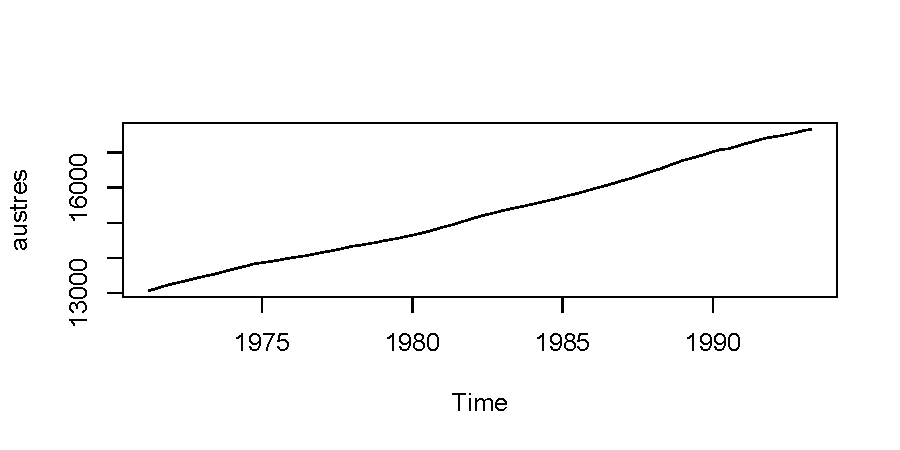
\includegraphics[width=.7\textwidth]{figure/pos-ts-02-1} 

}


\end{knitrout}

A different example, using data set  \Rdata{nottem} containing meteorological data for Nottingham, shows a clear cyclic component. The annual cycle of mean air temperatures (in degrees Fahrenheit) is clear when data are plotted.

\begin{knitrout}\footnotesize
\definecolor{shadecolor}{rgb}{0.969, 0.969, 0.969}\color{fgcolor}\begin{kframe}
\begin{alltt}
\hlkwd{data}\hlstd{(nottem)}
\hlkwd{is.ts}\hlstd{(nottem)}
\end{alltt}
\begin{verbatim}
## [1] TRUE
\end{verbatim}
\begin{alltt}
\hlkwd{plot}\hlstd{(nottem)}
\end{alltt}
\end{kframe}

{\centering 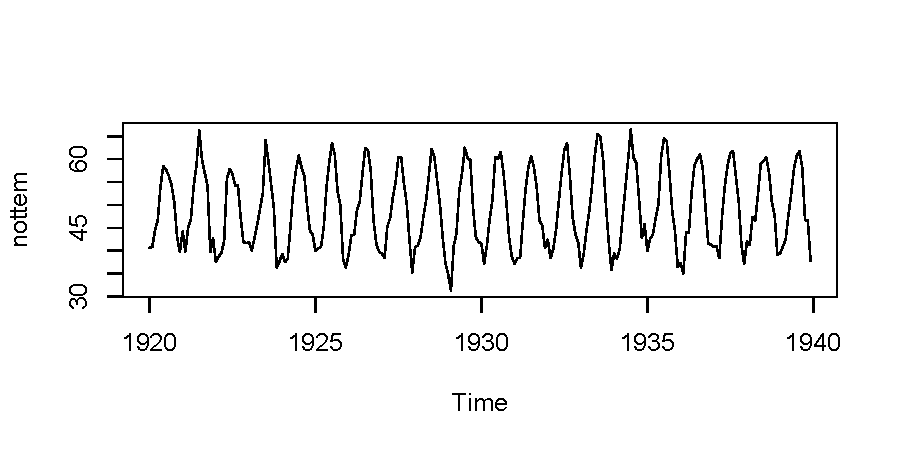
\includegraphics[width=.7\textwidth]{figure/pos-ts-03-1} 

}


\end{knitrout}

In\index{time series!decomposition} the next two code chunks, two different approaches to time series decomposition are used. In the first one we use a moving average to capture the trend, while in the second approach we use Loess (a smooth curve fitted by local weighted regression) for the decomposition, a method for which the acronym STL (Seasonal and Trend decomposition using Loess) is used.\qRfunction{decompose()}\qRfunction{stl()} Before decomposing the time-series we reexpress the temperatures in degrees Celsius.

\begin{knitrout}\footnotesize
\definecolor{shadecolor}{rgb}{0.969, 0.969, 0.969}\color{fgcolor}\begin{kframe}
\begin{alltt}
\hlstd{nottem.celcius} \hlkwb{<-} \hlstd{(nottem} \hlopt{-} \hlnum{32}\hlstd{)} \hlopt{*} \hlnum{5}\hlopt{/}\hlnum{9}
\end{alltt}
\end{kframe}
\end{knitrout}

We set the seasonal window to 7 months, the minimum accepted.


\begin{knitrout}\footnotesize
\definecolor{shadecolor}{rgb}{0.969, 0.969, 0.969}\color{fgcolor}\begin{kframe}
\begin{alltt}
\hlstd{nottem.stl} \hlkwb{<-} \hlkwd{stl}\hlstd{(nottem.celcius,} \hlkwc{s.window} \hlstd{=} \hlnum{7}\hlstd{)}
\hlkwd{plot}\hlstd{(nottem.stl)}
\end{alltt}
\end{kframe}

{\centering 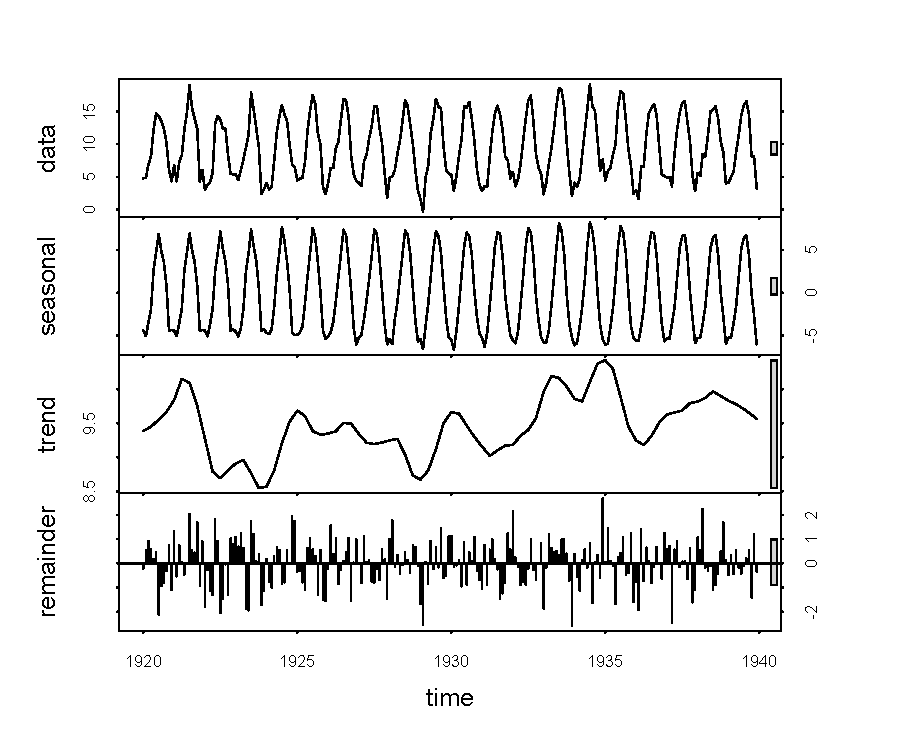
\includegraphics[width=.7\textwidth]{figure/pos-ts-05-1} 

}


\end{knitrout}

\begin{advplayground}
It is interesting to explore the class and structure of the object returned by \Rfunction{stl()}, as we may want to extract components. Run the statements below to find out, and then plot individual components from the time series decomposition.

\begin{knitrout}\footnotesize
\definecolor{shadecolor}{rgb}{0.969, 0.969, 0.969}\color{fgcolor}\begin{kframe}
\begin{alltt}
\hlkwd{class}\hlstd{(nottem.stl)}
\hlkwd{str}\hlstd{(nottem.stl)}
\end{alltt}
\end{kframe}
\end{knitrout}
\end{advplayground}

\index{time series|)}

\section{Multivariate statistics}\label{sec:stat:MV}
\index{multivariate methods|(}

\subsection{Multivariate analysis of variance}
\index{multivariate analysis of variance|(}
\index{MANOVA|see{multivariate analysis of variance}}
Multivariate methods take into account several response variables simultaneously, as part of a single analysis. In practice it is usual to use contributed packages for multivariate data analysis in \Rlang, except for simple cases. We will look first at \emph{multivariate} ANOVA or MANOVA. In the same way as \Rfunction{aov()} is a wrapper that uses internally \Rfunction{lm()}, \Rfunction{manova()} is a wrapper that uses internally \Rfunction{aov()}.

Multivariate model formulas in base \Rlang require the use of column binding (\code{cbind()}) on the left-hand side (lhs) of the model formula. For the next examples we use the well-known \Rdata{iris} data set, containing size measurements for flowers of two species of \emph{Iris}.

\begin{knitrout}\footnotesize
\definecolor{shadecolor}{rgb}{0.969, 0.969, 0.969}\color{fgcolor}\begin{kframe}
\begin{alltt}
\hlkwd{data}\hlstd{(iris)}
\hlstd{mmf1} \hlkwb{<-} \hlkwd{lm}\hlstd{(}\hlkwd{cbind}\hlstd{(Petal.Length, Petal.Width)} \hlopt{~}  \hlstd{Species,} \hlkwc{data} \hlstd{= iris)}
\hlkwd{anova}\hlstd{(mmf1)}
\end{alltt}
\begin{verbatim}
## Analysis of Variance Table
## 
##              Df  Pillai approx F num Df den Df    Pr(>F)    
## (Intercept)   1 0.98786   5939.2      2    146 < 2.2e-16 ***
## Species       2 1.04645     80.7      4    294 < 2.2e-16 ***
## Residuals   147                                             
## ---
## Signif. codes:  0 '***' 0.001 '**' 0.01 '*' 0.05 '.' 0.1 ' ' 1
\end{verbatim}
\begin{alltt}
\hlkwd{summary}\hlstd{(mmf1)}
\end{alltt}
\begin{verbatim}
## Response Petal.Length :
## 
## Call:
## lm(formula = Petal.Length ~ Species, data = iris)
## 
## Residuals:
##    Min     1Q Median     3Q    Max 
## -1.260 -0.258  0.038  0.240  1.348 
## 
## Coefficients:
##                   Estimate Std. Error t value Pr(>|t|)    
## (Intercept)        1.46200    0.06086   24.02   <2e-16 ***
## Speciesversicolor  2.79800    0.08607   32.51   <2e-16 ***
## Speciesvirginica   4.09000    0.08607   47.52   <2e-16 ***
## ---
## Signif. codes:  0 '***' 0.001 '**' 0.01 '*' 0.05 '.' 0.1 ' ' 1
## 
## Residual standard error: 0.4303 on 147 degrees of freedom
## Multiple R-squared:  0.9414,	Adjusted R-squared:  0.9406 
## F-statistic:  1180 on 2 and 147 DF,  p-value: < 2.2e-16
## 
## 
## Response Petal.Width :
## 
## Call:
## lm(formula = Petal.Width ~ Species, data = iris)
## 
## Residuals:
##    Min     1Q Median     3Q    Max 
## -0.626 -0.126 -0.026  0.154  0.474 
## 
## Coefficients:
##                   Estimate Std. Error t value Pr(>|t|)    
## (Intercept)        0.24600    0.02894    8.50 1.96e-14 ***
## Speciesversicolor  1.08000    0.04093   26.39  < 2e-16 ***
## Speciesvirginica   1.78000    0.04093   43.49  < 2e-16 ***
## ---
## Signif. codes:  0 '***' 0.001 '**' 0.01 '*' 0.05 '.' 0.1 ' ' 1
## 
## Residual standard error: 0.2047 on 147 degrees of freedom
## Multiple R-squared:  0.9289,	Adjusted R-squared:  0.9279 
## F-statistic:   960 on 2 and 147 DF,  p-value: < 2.2e-16
\end{verbatim}
\end{kframe}
\end{knitrout}

\begin{knitrout}\footnotesize
\definecolor{shadecolor}{rgb}{0.969, 0.969, 0.969}\color{fgcolor}\begin{kframe}
\begin{alltt}
\hlstd{mmf2} \hlkwb{<-} \hlkwd{manova}\hlstd{(}\hlkwd{cbind}\hlstd{(Petal.Length, Petal.Width)} \hlopt{~}  \hlstd{Species,} \hlkwc{data} \hlstd{= iris)}
\hlkwd{anova}\hlstd{(mmf2)}
\end{alltt}
\begin{verbatim}
## Analysis of Variance Table
## 
##              Df  Pillai approx F num Df den Df    Pr(>F)    
## (Intercept)   1 0.98786   5939.2      2    146 < 2.2e-16 ***
## Species       2 1.04645     80.7      4    294 < 2.2e-16 ***
## Residuals   147                                             
## ---
## Signif. codes:  0 '***' 0.001 '**' 0.01 '*' 0.05 '.' 0.1 ' ' 1
\end{verbatim}
\begin{alltt}
\hlkwd{summary}\hlstd{(mmf2)}
\end{alltt}
\begin{verbatim}
##            Df Pillai approx F num Df den Df    Pr(>F)    
## Species     2 1.0465   80.661      4    294 < 2.2e-16 ***
## Residuals 147                                            
## ---
## Signif. codes:  0 '***' 0.001 '**' 0.01 '*' 0.05 '.' 0.1 ' ' 1
\end{verbatim}
\end{kframe}
\end{knitrout}

\begin{advplayground}
Modify the example above to use \code{aov()} instead of \code{manova()} and save the result to a variable named \code{mmf3}.
Use \code{class()}, \code{attributes()}, \code{names()}, \code{str()} and extraction of members to explore objects \code{mmf1}, \code{mmf2} and \code{mmf3}. Are they different?
\end{advplayground}

\index{multivariate analysis of variance|)}

\subsection{Principal components analysis}\label{sec:stat:PCA}
\index{principal components analysis|(}\index{PCA|see {principal components analysis}}

Principal components analysis (PCA) is used to simplify a data set by combining variables with similar and ``mirror'' behavior into principal components. At a later stage, we frequently try to interpret these components in relation to known and/or assumed independent variables. Base \Rlang's function \Rfunction{prcomp()} computes the principal components and accepts additional arguments for centering and scaling.

\begin{knitrout}\footnotesize
\definecolor{shadecolor}{rgb}{0.969, 0.969, 0.969}\color{fgcolor}\begin{kframe}
\begin{alltt}
\hlstd{pc} \hlkwb{<-} \hlkwd{prcomp}\hlstd{(iris[}\hlkwd{c}\hlstd{(}\hlstr{"Sepal.Length"}\hlstd{,} \hlstr{"Sepal.Width"}\hlstd{,}
                    \hlstr{"Petal.Length"}\hlstd{,} \hlstr{"Petal.Width"}\hlstd{)],}
             \hlkwc{center} \hlstd{=} \hlnum{TRUE}\hlstd{,}
             \hlkwc{scale} \hlstd{=} \hlnum{TRUE}\hlstd{)}
\end{alltt}
\end{kframe}
\end{knitrout}

By printing the returned object we can see the loadings of each variable in the principal components \code{P1} to \code{P4}.
\begin{knitrout}\footnotesize
\definecolor{shadecolor}{rgb}{0.969, 0.969, 0.969}\color{fgcolor}\begin{kframe}
\begin{alltt}
\hlkwd{class}\hlstd{(pc)}
\end{alltt}
\begin{verbatim}
## [1] "prcomp"
\end{verbatim}
\begin{alltt}
\hlstd{pc}
\end{alltt}
\begin{verbatim}
## Standard deviations (1, .., p=4):
## [1] 1.7083611 0.9560494 0.3830886 0.1439265
## 
## Rotation (n x k) = (4 x 4):
##                     PC1         PC2        PC3        PC4
## Sepal.Length  0.5210659 -0.37741762  0.7195664  0.2612863
## Sepal.Width  -0.2693474 -0.92329566 -0.2443818 -0.1235096
## Petal.Length  0.5804131 -0.02449161 -0.1421264 -0.8014492
## Petal.Width   0.5648565 -0.06694199 -0.6342727  0.5235971
\end{verbatim}
\end{kframe}
\end{knitrout}

In the summary, the rows ``Proportion of Variance'' and ``Cumulative Proportion'' are most informative of the contribution of each principal component (PC) to explaining the variation among observations.

\begin{knitrout}\footnotesize
\definecolor{shadecolor}{rgb}{0.969, 0.969, 0.969}\color{fgcolor}\begin{kframe}
\begin{alltt}
\hlkwd{summary}\hlstd{(pc)}
\end{alltt}
\begin{verbatim}
## Importance of components:
##                           PC1    PC2     PC3     PC4
## Standard deviation     1.7084 0.9560 0.38309 0.14393
## Proportion of Variance 0.7296 0.2285 0.03669 0.00518
## Cumulative Proportion  0.7296 0.9581 0.99482 1.00000
\end{verbatim}
\end{kframe}
\end{knitrout}



Method \Rfunction{biplot()} produces a plot with one principal component (PC) on each axis, plus arrows for the loadings.

\begin{knitrout}\footnotesize
\definecolor{shadecolor}{rgb}{0.969, 0.969, 0.969}\color{fgcolor}\begin{kframe}
\begin{alltt}
\hlkwd{biplot}\hlstd{(pc)}
\end{alltt}
\end{kframe}

{\centering 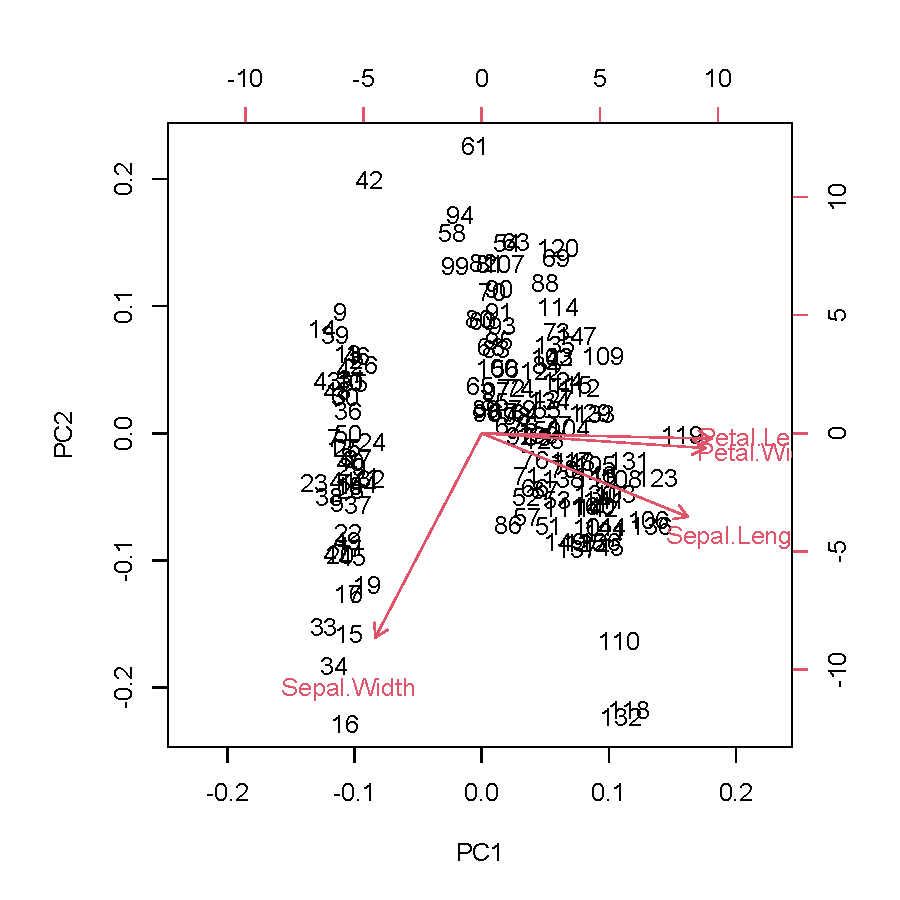
\includegraphics[width=.7\textwidth]{figure/pos-pca-05-1} 

}


\end{knitrout}



Method \code{plot()} generates a bar plot of variances corresponding to the different components.

\begin{knitrout}\footnotesize
\definecolor{shadecolor}{rgb}{0.969, 0.969, 0.969}\color{fgcolor}\begin{kframe}
\begin{alltt}
\hlkwd{plot}\hlstd{(pc)}
\end{alltt}
\end{kframe}

{\centering 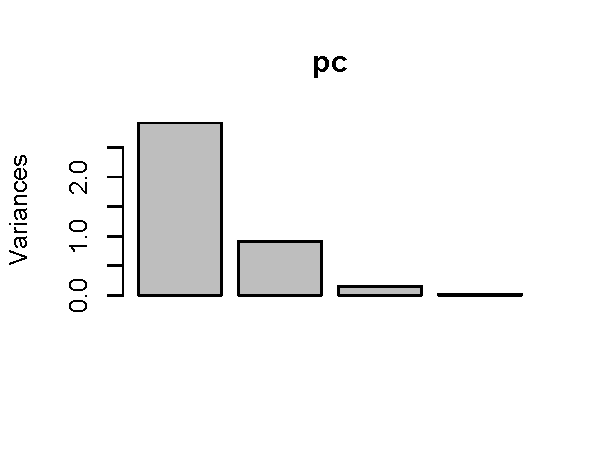
\includegraphics[width=.54\textwidth]{figure/pos-pca-04-1} 

}


\end{knitrout}

Visually more elaborate plots of the principal components and their loadings can be obtained using package \pkgnameNI{ggplot} described in chapter \ref{chap:R:plotting} starting on page \pageref{chap:R:plotting}. Package \pkgnameNI{ggfortify} extends \pkgnameNI{ggplot} so as to make it easy to plot principal components and their loadings.

\begin{playground}
For growth and morphological data, a log-transformation can be suitable given that variance is frequently proportional to the magnitude of the values measured. We leave as an exercise to repeat the above analysis using transformed values for the dimensions of petals and sepals. How much does the use of transformations change the outcome of the analysis?
\end{playground}

\begin{advplayground}
As for other fitted models, the object returned by function \Rfunction{prcomp()} is a list with multiple components.

\begin{knitrout}\footnotesize
\definecolor{shadecolor}{rgb}{0.969, 0.969, 0.969}\color{fgcolor}\begin{kframe}
\begin{alltt}
\hlkwd{str}\hlstd{(pc,} \hlkwc{max.level} \hlstd{=} \hlnum{1}\hlstd{)}
\end{alltt}
\end{kframe}
\end{knitrout}
\end{advplayground}

\index{principal components analysis|)}

\subsection{Multidimensional scaling}\label{sec:stat:MDS}
\index{multidimensional scaling|(}\index{MDS|see {multidimensional scaling}}

The aim of multidimensional scaling (MDS) is to visualize in 2D space the similarity between pairs of observations. The values for the observed variable(s) are used to compute a measure of distance among pairs of observations. The nature of the data will influence what distance metric is most informative.
For MDS we start with a matrix of distances among observations. We will use, for the example, distances in kilometers between geographic locations in Europe from data set \Rdata{eurodist}.

\begin{knitrout}\footnotesize
\definecolor{shadecolor}{rgb}{0.969, 0.969, 0.969}\color{fgcolor}\begin{kframe}
\begin{alltt}
\hlstd{loc} \hlkwb{<-} \hlkwd{cmdscale}\hlstd{(eurodist)}
\end{alltt}
\end{kframe}
\end{knitrout}

We can see that the returned object \code{loc} is a \code{matrix}, with names for one of the dimensions.

\begin{knitrout}\footnotesize
\definecolor{shadecolor}{rgb}{0.969, 0.969, 0.969}\color{fgcolor}\begin{kframe}
\begin{alltt}
\hlkwd{class}\hlstd{(loc)}
\end{alltt}
\begin{verbatim}
## [1] "matrix" "array"
\end{verbatim}
\begin{alltt}
\hlkwd{dim}\hlstd{(loc)}
\end{alltt}
\begin{verbatim}
## [1] 21  2
\end{verbatim}
\begin{alltt}
\hlkwd{dimnames}\hlstd{(loc)}
\end{alltt}
\begin{verbatim}
## [[1]]
##  [1] "Athens"          "Barcelona"       "Brussels"        "Calais"         
##  [5] "Cherbourg"       "Cologne"         "Copenhagen"      "Geneva"         
##  [9] "Gibraltar"       "Hamburg"         "Hook of Holland" "Lisbon"         
## [13] "Lyons"           "Madrid"          "Marseilles"      "Milan"          
## [17] "Munich"          "Paris"           "Rome"            "Stockholm"      
## [21] "Vienna"         
## 
## [[2]]
## NULL
\end{verbatim}
\begin{alltt}
\hlkwd{head}\hlstd{(loc)}
\end{alltt}
\begin{verbatim}
##                 [,1]      [,2]
## Athens    2290.27468 1798.8029
## Barcelona -825.38279  546.8115
## Brussels    59.18334 -367.0814
## Calais     -82.84597 -429.9147
## Cherbourg -352.49943 -290.9084
## Cologne    293.68963 -405.3119
\end{verbatim}
\end{kframe}
\end{knitrout}

To make the code easier to read, two vectors are first extracted from the matrix and named \code{x} and \code{y}. We force aspect to equality so that distances on both axes are comparable.



\begin{knitrout}\footnotesize
\definecolor{shadecolor}{rgb}{0.969, 0.969, 0.969}\color{fgcolor}\begin{kframe}
\begin{alltt}
\hlstd{x} \hlkwb{<-} \hlstd{loc[,} \hlnum{1}\hlstd{]}
\hlstd{y} \hlkwb{<-} \hlopt{-}\hlstd{loc[,} \hlnum{2}\hlstd{]} \hlcom{# change sign so North is at the top}
\hlkwd{plot}\hlstd{(x, y,} \hlkwc{type} \hlstd{=} \hlstr{"n"}\hlstd{,} \hlkwc{asp} \hlstd{=} \hlnum{1}\hlstd{,}
     \hlkwc{main} \hlstd{=} \hlstr{"cmdscale(eurodist)"}\hlstd{)}
\hlkwd{text}\hlstd{(x, y,} \hlkwd{rownames}\hlstd{(loc),} \hlkwc{cex} \hlstd{=} \hlnum{0.6}\hlstd{)}
\end{alltt}
\end{kframe}

{\centering 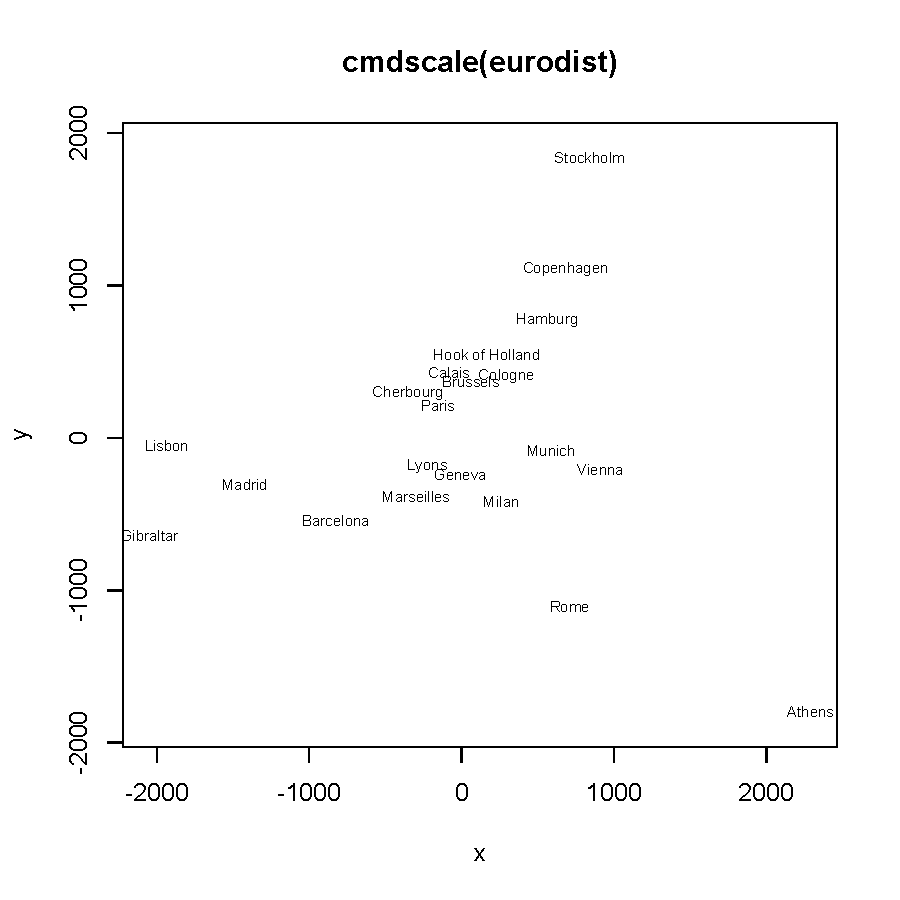
\includegraphics[width=.7\textwidth]{figure/pos-mds-03-1} 

}


\end{knitrout}

\begin{advplayground}
  Find data on the mean annual temperature, mean annual rainfall and mean number of sunny days at each of the locations in the \code{eurodist} data set. Next, compute suitable distance metrics, for example, using function \Rfunction{dist}. Finally, use MDS to visualize how similar the locations are with respect to each of the three variables. Devise a measure of distance that takes into account the three climate variables and use MDS to find how distant the different locations are.
\end{advplayground}

\index{multidimensional scaling|)}

\subsection{Cluster analysis}\label{sec:stat:cluster}
\index{cluster analysis|(}

In cluster analysis, the aim is to group observations into discrete groups with maximal internal homogeneity and maximum group-to-group differences. In the next example we use function \Rfunction{hclust()} from the base-\Rlang package \pkgname{stats}. We use, as above, the \Rdata{eurodist} data which directly provides distances. In other cases a matrix of distances between pairs of observations needs to be first calculated with function \Rfunction{dist} which supports several methods.

\begin{knitrout}\footnotesize
\definecolor{shadecolor}{rgb}{0.969, 0.969, 0.969}\color{fgcolor}\begin{kframe}
\begin{alltt}
\hlstd{hc} \hlkwb{<-} \hlkwd{hclust}\hlstd{(eurodist)}
\hlkwd{print}\hlstd{(hc)}
\end{alltt}
\begin{verbatim}
## 
## Call:
## hclust(d = eurodist)
## 
## Cluster method   : complete 
## Number of objects: 21
\end{verbatim}
\end{kframe}
\end{knitrout}

\begin{knitrout}\footnotesize
\definecolor{shadecolor}{rgb}{0.969, 0.969, 0.969}\color{fgcolor}\begin{kframe}
\begin{alltt}
\hlkwd{plot}\hlstd{(hc)}
\end{alltt}
\end{kframe}

{\centering 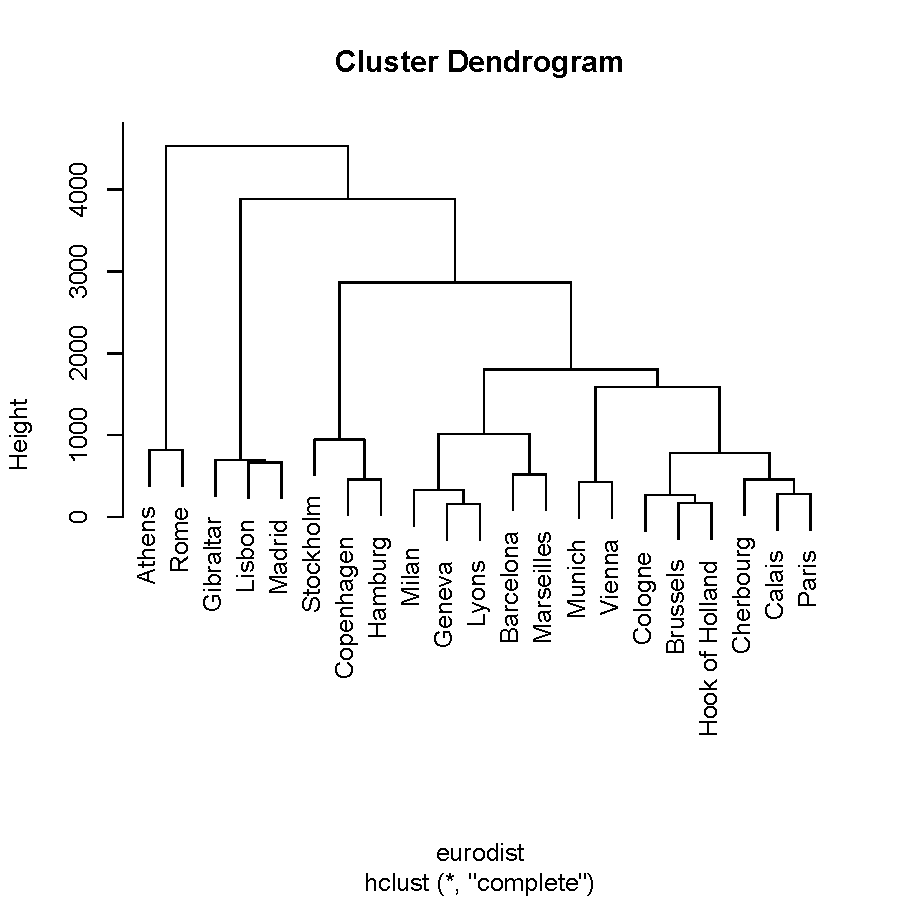
\includegraphics[width=.7\textwidth]{figure/pos-cluster-02-1} 

}


\end{knitrout}

We can use \Rfunction{cutree()} to limit the number of clusters by directly passing as an argument the desired number of clusters or the height at which to cut the tree.

\begin{knitrout}\footnotesize
\definecolor{shadecolor}{rgb}{0.969, 0.969, 0.969}\color{fgcolor}\begin{kframe}
\begin{alltt}
\hlkwd{cutree}\hlstd{(hc,} \hlkwc{k} \hlstd{=} \hlnum{5}\hlstd{)}
\end{alltt}
\begin{verbatim}
##          Athens       Barcelona        Brussels          Calais       Cherbourg 
##               1               2               3               3               3 
##         Cologne      Copenhagen          Geneva       Gibraltar         Hamburg 
##               3               4               2               5               4 
## Hook of Holland          Lisbon           Lyons          Madrid      Marseilles 
##               3               5               2               5               2 
##           Milan          Munich           Paris            Rome       Stockholm 
##               2               3               3               1               4 
##          Vienna 
##               3
\end{verbatim}
\end{kframe}
\end{knitrout}

The object returned by \Rfunction{hclust()} contains details of the result of the clustering, which allows further manipulation and plotting.
\begin{knitrout}\footnotesize
\definecolor{shadecolor}{rgb}{0.969, 0.969, 0.969}\color{fgcolor}\begin{kframe}
\begin{alltt}
\hlkwd{str}\hlstd{(hc)}
\end{alltt}
\begin{verbatim}
## List of 7
##  $ merge      : int [1:20, 1:2] -8 -3 -6 -4 -16 -17 -5 -7 -2 -12 ...
##  $ height     : num [1:20] 158 172 269 280 328 428 460 460 521 668 ...
##  $ order      : int [1:21] 1 19 9 12 14 20 7 10 16 8 ...
##  $ labels     : chr [1:21] "Athens" "Barcelona" "Brussels" "Calais" ...
##  $ method     : chr "complete"
##  $ call       : language hclust(d = eurodist)
##  $ dist.method: NULL
##  - attr(*, "class")= chr "hclust"
\end{verbatim}
\end{kframe}
\end{knitrout}

\index{cluster analysis|)}

%\subsection{Discriminant analysis}\label{sec:stat:DA}
%\index{discriminant analysis|(}
%
%In discriminant analysis the categories or groups to which objects belong are known \emph{a priori} for a training data set. The aim is to fit/build a classifier that will allow us to assign future observations to the different non-overlapping groups with as few mistakes as possible.
%
%
%\index{discriminant analysis|)}
\index{multivariate methods|)}

\section{Further reading}\label{sec:stat:further:reading}

Two recent text books\index{further reading!statistics in R} on statistics, following a modern approach, and using \Rlang for examples, are \citetitle{Diez2019} \autocite{Diez2019} and \citetitle{Holmes2019} \autocite{Holmes2019}. Three examples of books introducing statistical computations in \Rlang are \citetitle{Dalgaard2008} \autocite{Dalgaard2008}, \citetitle{Everitt2009} \autocite{Everitt2009} and \citetitle{Zuur2009} \autocite{Zuur2009}. More advanced books are available with detailed descriptions of various types of analyses in \Rlang, including thorough descriptions of the methods briefly presented in this chapter. Good examples of books with broad scope are \citebooktitle{Crawley2012} \autocite{Crawley2012} and the classic reference \citebooktitle{Venables2002} \autocite{Venables2002}. More specific books are also available from which a few suggestions for further reading are \citebooktitle{Everitt2011} \autocite{Everitt2011}, \citebooktitle{Faraway2004} \autocite{Faraway2004}, \citebooktitle{Faraway2006} \autocite{Faraway2006}, \citebooktitle{Pinheiro2000} \autocite{Pinheiro2000} and \citebooktitle{Wood2017} \autocite{Wood2017}.









\backmatter

\printbibliography

\printindex

\printindex[rcatsidx]

\printindex[rindex]

\end{document}

\appendix

\chapter{Build information}

\begin{knitrout}\footnotesize
\definecolor{shadecolor}{rgb}{0.969, 0.969, 0.969}\color{fgcolor}\begin{kframe}
\begin{alltt}
\hlkwd{Sys.info}\hlstd{()}
\end{alltt}
\end{kframe}
\end{knitrout}



\begin{knitrout}\footnotesize
\definecolor{shadecolor}{rgb}{0.969, 0.969, 0.969}\color{fgcolor}\begin{kframe}
\begin{alltt}
\hlkwd{sessionInfo}\hlstd{()}
\end{alltt}
\end{kframe}
\end{knitrout}

\end{document}


